\documentclass{plantilla}

\usepackage{multirow}
\usepackage{siunitx}
\usepackage{array}
\usepgfplotslibrary{fillbetween}

\sisetup{
    output-decimal-marker = {,},
    group-digits = none,
    per-mode = symbol
}
\DeclareSIUnit{\ohm}{\ensuremath{\Omega}}

% Datos de cátedra y grupo
\materia{Electrónica Aplicada II}
\comision{4R2}
\titulo{Trabajo Práctico N$^{\circ}$6: Fuente de Alimentación Lineal con Regulador Integrado LM7805 y Etapa Prereguladora Serie (Consigna 6)}
\autores{Ernst Pedro (400624), López Demichelis Alejo (401900),\\ Polizze Tomás (400793), Rao Valentino (402308)}

\begin{document}

\maketitle

\begin{abstract}
En el presente informe técnico se desarrolla el diseño analítico, el dimensionamiento electrotérmico y la verificación mediante simulación circuital SPICE de la Consigna 6 correspondiente a la Unidad 6 (Fuentes de Alimentación de Baja Potencia). El sistema parte de una fuente primaria de corriente continua de \SI{25}{\volt} y emplea un regulador monolítico fijo de tres terminales \texttt{LM7805C} (\SI{5}{\volt}). Con el propósito de optimizar la regulación del voltaje de línea, atenuar el rizado de entrada y aliviar el estrés térmico del circuito integrado, se diseña una etapa prereguladora lineal serie discreta basada en un seguidor por emisor NPN (\texttt{TIP31C}) y referencia Zener (\texttt{1N5240B}/\texttt{1N4740A} de \SI{10}{\volt}), acotando la tensión de entrada al regulador integrado estrictamente dentro de la ventana óptima recomendada por el fabricante ($V_{i,\text{reg}} \in [\SI{8}{\volt}, \SI{12}{\volt}]$). Se contrasta mediante simulación el desempeño de la regulación de línea para $V_{in} = \SI{25}{\volt}$ y $V_{in} = \SI{10}{\volt}$ tanto con etapa prereguladora como sin ella, verificando el punto de operación del transistor de paso dentro del Área de Operación Segura (SOA), calculando los disipadores térmicos requeridos y determinando la totalidad de los parámetros de calidad de la fuente ($R_{\text{red}}$, $R_{\text{car}}$, $R_{\text{sal}}$, $C.T.$, $V_{r,\text{pp}}$, $V_{\text{ef,rip}}$, $RR$ y rendimiento $\eta$).
\end{abstract}

\begin{IEEEkeywords}
Fuente de alimentación lineal, regulador integrado LM7805, etapa prereguladora Zener, regulación de línea, Área de Operación Segura (SOA), resistencia térmica, disipador de calor, factores de calidad.
\end{IEEEkeywords}

\section{Introducción y Planteo del Problema}

\subsection{Enunciado de la Consigna 6}
El presente trabajo aborda la resolución integral de la \textbf{Consigna 6} de la evaluación práctica de la Unidad 6 (\emph{Fuentes de Alimentación}):
\begin{quote}
\emph{``Diseñar y calcular una fuente de alimentación con un regulador lineal integrado LM7805. Se dispone de una fuente primaria de \SI{25}{\volt} dc. A los fines de mejorar la regulación del voltaje de línea es necesario un rango de $V_{in} = \SI{8}{\volt}\text{--}\SI{12}{\volt}$. Incluir en el diseño una etapa que cumpla con este objetivo. Verificar mediante simulación la regulación de línea para $V_{in} = \SI{25}{\volt}$ y $V_{in} = \SI{10}{\volt}$. Seleccionar Transistor, verificar punto de operación según SOA e incluir eventual cálculo de disipador. Obtener todos los parámetros de Calidad de fuentes de alimentación.''}
\end{quote}

\subsection{Arquitectura Interna y Protecciones del Regulador LM7805C}
Los reguladores monolíticos fijos de tres terminales de la familia \texttt{LM78XX} (y su equivalente directo $\mu\text{A78XXC}$) integran en un único chip de silicio la totalidad de los bloques funcionales de un regulador lineal serie con realimentación negativa, añadiendo circuitos internos de autoprotección \cite{gonzalez_p3}. Como se esquematiza en el diagrama en bloques de la Figura~\ref{fig:bloques_7805} (basado en las Figuras 6-55 a 6-57 del material de cátedra), la estructura interna comprende:
\begin{enumerate}
    \item \textbf{Elemento regulador serie de paso ($Q_1\text{--}Q_2$):} Configurado como un par compuesto Darlington NPN capaz de manejar corrientes continuas de salida de hasta $I_{O,\max} = \SI{1,0}{\ampere}$ (con picos de hasta \SI{2,2}{\ampere}) presentando una tensión mínima de caída entrada-salida (\emph{dropout voltage}) $V_{DO} = V_I - V_O \approx \SI{2,0}{\volt}$.
    \item \textbf{Referencia de tensión interna ($V_{\text{ref}}$):} Basada en referencia de banda prohibida (\emph{bandgap}) o Zener compensado térmicamente ($D_1, Q_3$), polarizada mediante fuentes de corriente constantes internas para independizar la tensión de referencia respecto de fluctuaciones en la tensión de entrada $V_I$.
    \item \textbf{Red de muestreo ($R_1, R_2$) y amplificador de error:} El divisor resistivo interno toma una fracción proporcional a la tensión de salida $V_O$ y la compara en un amplificador diferencial con $V_{\text{ref}}$, ajustando continuamente la excitación de base del par Darlington para mantener $V_O = \SI{5,0}{\volt}$.
    \item \textbf{Circuito limitador de corriente constante ($R_{CL}, Q_4$):} Cuando la caída de tensión en la resistencia sensora $R_{CL}$ alcanza el umbral de conducción base-emisor del transistor $Q_4$ ($V_{BE(Q_4)} \approx \SI{0,65}{\volt}$), éste drena corriente desde la base del Darlington serie, limitando la corriente de salida ante sobrecargas o cortocircuitos francos.
    \item \textbf{Protección de Área de Operación Segura (SOA) ($D_2, R_3, R_4$):} Cuando la diferencia de potencial entrada-salida $(V_I - V_O)$ supera la tensión de ruptura del diodo Zener interno $D_2$, circula una corriente adicional proporcional a $(V_I - V_O)$ a través de $R_3$ y $R_4$ hacia la base de $Q_4$. Ello anticipa la saturación de $Q_4$ (limitación tipo \emph{foldback}), reduciendo la corriente máxima que puede suministrar el integrado cuando trabaja con alta tensión diferencial $(V_I - V_O)$, tal como se verifica en la curva de corriente pico de la hoja de datos (Fig. 6-58 de \cite{gonzalez_p3}).
    \item \textbf{Corte térmico por sobretemperatura ($Q_3$):} Un transistor sensor ubicado físicamente adyacente al par de potencia $Q_1\text{--}Q_2$ se encuentra polarizado con una tensión base-emisor fija de aproximadamente \SI{0,4}{\volt} (insuficiente para conducir a \SI{25}{\celsius}). Debido al coeficiente térmico negativo de la juntura ($\approx \SI{-2}{\milli\volt\per\celsius}$), si la temperatura de juntura alcanza el umbral crítico de \SI{150}{\celsius} a \SI{190}{\celsius}, $Q_3$ entra en saturación y anula la corriente de excitación del paso serie, incorporando histéresis térmica para prevenir oscilaciones.
\end{enumerate}

\begin{figure}[htbp]
\centering
\resizebox{\columnwidth}{!}{%
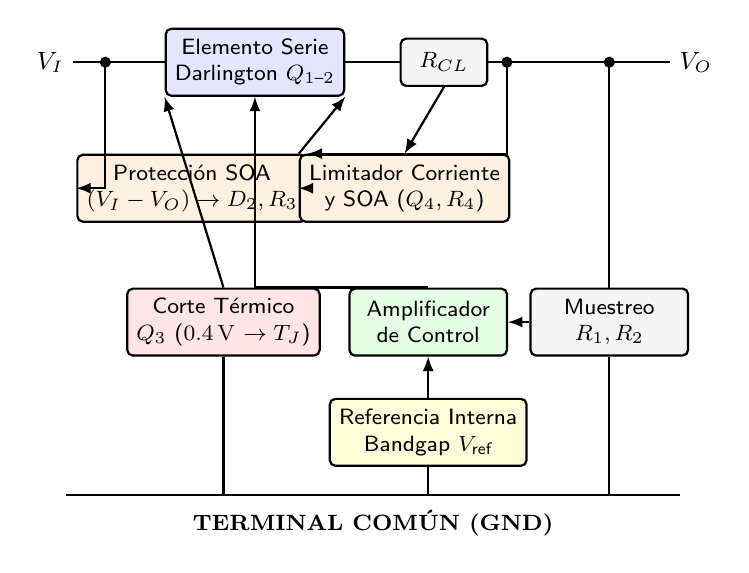
\begin{tikzpicture}[
    block/.style={draw, thick, rectangle, rounded corners=2pt, minimum height=0.85cm, minimum width=2.0cm, align=center, font=\footnotesize\sffamily, fill=gray!8},
    sum/.style={draw, thick, circle, inner sep=1.5pt, font=\footnotesize},
    line/.style={thick, -latex}
]
    % Nodos de entrada y salida
    \node (vin) at (0, 2.5) [font=\small\bfseries] {$V_I$};
    \node (vout) at (8.2, 2.5) [font=\small\bfseries] {$V_O$};

    % Elemento serie y Rsc
    \node[block, fill=blue!10] (pass) at (2.6, 2.5) {Elemento Serie\\Darlington $Q_{1\text{--}2}$};
    \node[block, minimum width=1.1cm, minimum height=0.6cm] (rsc) at (5.0, 2.5) {$R_{CL}$};

    % Protecciones superiores
    \node[block, fill=orange!12] (soa) at (1.8, 0.9) {Protección SOA\\$(V_I - V_O) \to D_2, R_3$};
    \node[block, fill=orange!12] (ilim) at (4.5, 0.9) {Limitador Corriente\\y SOA ($Q_4, R_4$)};

    % Control, referencia, muestreo y térmica
    \node[block, fill=red!10] (therm) at (2.2, -0.8) {Corte Térmico\\$Q_3$ (\SI{0,4}{\volt} $\to T_J$)};
    \node[block, fill=green!10] (ctrl) at (4.8, -0.8) {Amplificador\\de Control};
    \node[block, fill=yellow!15] (vref) at (4.8, -2.2) {Referencia Interna\\Bandgap $V_{\text{ref}}$};
    \node[block] (samp) at (7.1, -0.8) {Muestreo\\$R_1, R_2$};

    % Conexiones principales
    \draw[thick] (vin) -- (pass.west);
    \draw[thick] (pass.east) -- (rsc.west);
    \draw[thick] (rsc.east) -- (vout);
    \draw[thick] (7.1, 2.5) -- (samp.north);
    \filldraw (7.1, 2.5) circle (1.8pt);
    \filldraw (0.7, 2.5) circle (1.8pt);

    % Conexiones de control y protecciones
    \draw[line] (0.7, 2.5) |- (soa.west);
    \draw[line] (5.8, 2.5) |- (soa.north east);
    \filldraw (5.8, 2.5) circle (1.8pt);
    \draw[line] (soa.east) -- (ilim.west);
    \draw[line] (rsc.south) -- (ilim.north);
    \draw[line] (ilim.north west) -- (pass.south east);

    \draw[line] (samp.west) -- (ctrl.east);
    \draw[line] (vref.north) -- (ctrl.south);
    \draw[line] (ctrl.north) -| (pass.south);
    \draw[line] (therm.north) -- (pass.south west);

    % Línea de masa común (GND)
    \draw[thick] (0.2, -3.0) -- (8.0, -3.0);
    \draw[thick] (therm.south) -- (2.2, -3.0);
    \draw[thick] (vref.south) -- (4.8, -3.0);
    \draw[thick] (samp.south) -- (7.1, -3.0);
    \node at (4.1, -3.35) [font=\footnotesize\bfseries] {TERMINAL COMÚN (GND)};
\end{tikzpicture}%
}
\caption{Diagrama funcional en bloques del regulador monolítico \texttt{LM7805C}, destacando el lazo de regulación y las protecciones de corriente, SOA y temperatura (adaptado de Figs. 6-55 y 6-57 \cite{gonzalez_p3}).}
\label{fig:bloques_7805}
\end{figure}

\subsection{Análisis de la Hoja de Datos y Fundamentación del Rango $V_{in(\text{reg})} = \SI{8}{\volt}\text{--}\SI{12}{\volt}$}
En la Tabla~\ref{tab:datasheet_7805} se sintetizan los parámetros eléctricos y térmicos relevantes del regulador $\mu\text{A7805C}$ / \texttt{LM7805C} en encapsulado TO-220, extraídos de la Figura 6-59 del material teórico \cite{gonzalez_p3, ti_7805}. Dichos parámetros se especifican en la condición nominal de ensayo $V_I = \SI{10}{\volt}$, $I_O = \SI{500}{\milli\ampere}$ y $T_J = \SI{25}{\celsius}$.

\begin{table}[htbp]
\centering
\caption{Características eléctricas y térmicas del regulador \texttt{LM7805C} ($\mu\text{A7805C}$, encapsulado TO-220) \cite{gonzalez_p3}.}
\label{tab:datasheet_7805}
\resizebox{\columnwidth}{!}{%
\begin{tabular}{llccc}
\toprule
\textbf{Parámetro} & \textbf{Condiciones de ensayo} & \textbf{Mín.} & \textbf{Típ.} & \textbf{Máx.} \\
\midrule
Tensión de salida ($V_O$) & $I_O = \SI{5}{\milli\ampere}\text{ a }\SI{1}{\ampere}, T_J = \SI{25}{\celsius}$ & \SI{4,8}{\volt} & \SI{5,0}{\volt} & \SI{5,2}{\volt} \\
Tensión de entrada ($V_I$) & Rango operativo recomendado & \SI{7,0}{\volt} & \SI{10,0}{\volt} & \SI{25,0}{\volt} \\
\textbf{Regulación de línea} & $V_I = \SI{7}{\volt}\text{ a }\SI{25}{\volt}, T_J = \SI{25}{\celsius}$ & --- & \textbf{\SI{3}{\milli\volt}} & \textbf{\SI{100}{\milli\volt}} \\
\textbf{Regulación de línea} & $\mathbf{V_I = \SI{8}{\volt}\text{ \textbf{a} }\SI{12}{\volt}}, T_J = \SI{25}{\celsius}$ & --- & \textbf{\SI{1}{\milli\volt}} & \textbf{\SI{50}{\milli\volt}} \\
Rechazo de ripple ($RR$) & $V_I = \SI{8}{\volt}\text{ a }\SI{18}{\volt}, f = \SI{120}{\hertz}$ & \SI{62}{\deci\bel} & \SI{78}{\deci\bel} & --- \\
Regulación de carga & $I_O = \SI{5}{\milli\ampere}\text{ a }\SI{1,5}{\ampere}, T_J = \SI{25}{\celsius}$ & --- & \SI{15}{\milli\volt} & \SI{100}{\milli\volt} \\
Regulación de carga & $I_O = \SI{250}{\milli\ampere}\text{ a }\SI{750}{\milli\ampere}$ & --- & \SI{5}{\milli\volt} & \SI{50}{\milli\volt} \\
Resistencia de salida ($r_o$) & $f = \SI{1}{\kilo\hertz}, T_J = \SI{0}{\celsius}\text{ a }\SI{125}{\celsius}$ & --- & \SI{0,017}{\ohm} & --- \\
Coeficiente térmico ($\Delta V_O/\Delta T$) & $I_O = \SI{5}{\milli\ampere}, T_J = \SI{0}{\celsius}\text{ a }\SI{125}{\celsius}$ & --- & \SI{-1,1}{\milli\volt\per\celsius} & --- \\
Tensión de \emph{dropout} ($V_{DO}$) & $I_O = \SI{1,0}{\ampere}, T_J = \SI{25}{\celsius}$ & --- & \SI{2,0}{\volt} & --- \\
Corriente de reposo ($I_d$) & $T_J = \SI{25}{\celsius}$ & --- & \SI{4,2}{\milli\ampere} & \SI{8,0}{\milli\ampere} \\
Variación de $I_d$ ($\Delta I_d$) & $V_I = \SI{7}{\volt}\text{ a }\SI{25}{\volt}$ / $I_O = \SI{5}{\milli\ampere}\text{ a }\SI{1}{\ampere}$ & --- & --- & \SI{1,3}{\milli\ampere} / \SI{0,5}{\milli\ampere} \\
Corriente de cortocircuito ($I_{SC}$) & $T_J = \SI{25}{\celsius}$ & --- & \SI{750}{\milli\ampere} & --- \\
Temperatura de juntura ($T_J$) & Rango operativo / Máx. absoluta & \SI{0}{\celsius} & --- & \SI{125}{\celsius} / \SI{150}{\celsius} \\
Resistencia térmica ($\theta_{JC} / \theta_{JA}$) & Encapsulado TO-220 (KCS / KC) & --- & \SI{3,0}{\celsius\per\watt} & \SI{19}{\celsius\per\watt}\text{--}\SI{65}{\celsius\per\watt} \\
\bottomrule
\end{tabular}%
}
\end{table}

El análisis detenido de la Tabla~\ref{tab:datasheet_7805} y de la Sección 6-9-3 del apunte de cátedra \cite{gonzalez_p3} justifica técnica y cuantitativamente por qué no resulta conveniente aplicar los \SI{25}{\volt} de la fuente primaria de manera directa al terminal de entrada del \texttt{LM7805C}, sino que debe incorporarse una etapa previa que sitúe su tensión de entrada $V_{i,\text{reg}}$ dentro del intervalo $[\SI{8}{\volt}, \SI{12}{\volt}]$:
\begin{itemize}
    \item \textbf{Optimización de la regulación de línea estática y dinámica:} Cuando el integrado opera dentro de la ventana central $\SI{8}{\volt} \le V_{i,\text{reg}} \le \SI{12}{\volt}$ (centrada en $V_{i,\text{reg}} \approx \SI{9,5}{\volt}\text{--}\SI{10,0}{\volt}$), la variación de tensión de salida se reduce de \SI{3}{\milli\volt} a \textbf{\SI{1}{\milli\volt} típico} (y el máximo garantizado se reduce a la mitad, de \SI{100}{\milli\volt} a \SI{50}{\milli\volt}). Más aún, dado que la etapa prereguladora estabiliza $V_{i,\text{reg}}$ mediante una referencia Zener, una variación severa en la línea primaria (por ejemplo de \SI{25}{\volt} a \SI{10}{\volt}, $\Delta V_{in} = \SI{15}{\volt}$, o fluctuaciones del $\pm \SI{10}{\percent}$ en torno a \SI{25}{\volt}) se traduce en una variación mínima sobre el nodo $V_{i,\text{reg}}$, logrando un doble efecto regulador en cascada.
    \item \textbf{Margen seguro sobre la tensión de \emph{dropout}:} El límite inferior de \SI{8,0}{\volt} asegura una caída diferencial entrada-salida en el regulador integrado de $V_{i,\text{reg}} - V_O = \SI{8,0}{\volt} - \SI{5,0}{\volt} = \SI{3,0}{\volt} > V_{DO} = \SI{2,0}{\volt}$, impidiendo que el transistor Darlington interno salga de su zona activa incluso ante valles de rizado.
    \item \textbf{Desacoplo térmico y preservación del SOA interno del CI:} Operando directamente a $V_{in} = \SI{25}{\volt}$, el diferencial sobre el \texttt{LM7805C} es $V_{in} - V_O = \SI{20}{\volt}$ (situado exactamente en el límite máximo de condiciones recomendadas de la Tabla~\ref{tab:datasheet_7805}). A una corriente nominal de $I_L = \SI{500}{\milli\ampere}$, el integrado debería disipar $P_{D(\text{7805})} = \SI{20}{\volt} \times \SI{0,5}{\ampere} = \SI{10,0}{\watt}$ (y \SI{20,0}{\watt} para $I_L = \SI{1,0}{\ampere}$), lo cual activa la limitación SOA interna ($D_2$) degradando la capacidad de corriente, además de inducir un fuerte corrimiento térmico de la tensión de salida ($\Delta V_O = \SI{-1,1}{\milli\volt\per\celsius} \cdot \Delta T_J$). Al reducir $V_{i,\text{reg}}$ a $\approx \SI{9,5}{\volt}$, la disipación en el \texttt{LM7805C} cae en más de un \SI{77}{\percent} (a sólo \SI{2,27}{\watt} para \SI{500}{\milli\ampere}), transfiriendo el esfuerzo térmico hacia un transistor discreto externo de potencia fácil de refrigerar.
\end{itemize}

\section{Diseño de la Etapa Prereguladora Serie}

\subsection{Selección y Justificación de la Topología Prereguladora}
Cuando la tensión provista por la fuente primaria ($V_{in} = \SI{25}{\volt}$) supera el rango óptimo de entrada del regulador monolítico ($V_{i,\text{reg}} \in [\SI{8}{\volt}, \SI{12}{\volt}]$), la Sección 6-9-5g del material de cátedra \cite{gonzalez_p3} presenta dos configuraciones circuitales posibles basadas en un transistor bipolar de paso serie $Q_1$ y un diodo Zener $D_Z$:
\begin{enumerate}
    \item \textbf{Topología de sustracción fija (Figura 6-72 de \cite{gonzalez_p3}):} Ubica al diodo Zener entre el colector (entrada $V_{in}$) y la base de $Q_1$, polarizándolo mediante un resistor hacia el emisor. La tensión resultante a la entrada del regulador integrado responde a la expresión:
    \begin{equation}
        V_{i,\text{reg}} \approx V_{in} - \left( V_Z + V_{BE(Q_1)} \right)
        \label{eq:topologia_descartada}
    \end{equation}
    Si bien esta configuración reduce el valor continuo de $V_{i,\text{reg}}$ cuando $V_{in} = \SI{25}{\volt}$ (adoptando por ejemplo $V_Z = \SI{14}{\volt}$ para obtener $V_{i,\text{reg}} \approx \SI{10}{\volt}$), adolece de dos limitaciones críticas para los requerimientos de la Consigna 6:
    \begin{itemize}
        \item En primer lugar, al derivar la expresión~\eqref{eq:topologia_descartada} respecto de $V_{in}$ resulta $\Delta V_{i,\text{reg}} \approx \Delta V_{in}$; es decir, traslada íntegramente el \SI{100}{\percent} de las variaciones de tensión de línea y de ripple de la fuente primaria hacia la entrada del \texttt{LM7805C}.
        \item En segundo término, al verificar la regulación de línea reduciendo la fuente primaria a $V_{in} = \SI{10}{\volt}$, resulta $V_{in} < V_Z + V_{BE(Q_1)}$, con lo cual el diodo Zener se apaga, el transistor $Q_1$ entra en corte y la fuente deja de funcionar por completo.
    \end{itemize}

    \item \textbf{Topología seguidor por emisor con referencia Zener a masa (Figura 6-71 de \cite{gonzalez_p3} y Figura 6-36 de \cite{gonzalez_p2}):} Conecta el cátodo del diodo Zener $D_Z$ a la base de $Q_1$ y su ánodo al terminal común de masa (GND), alimentándolo desde $V_{in}$ a través del resistor limitador $R_Z$. Aplicando la ley de tensiones de Kirchhoff en la malla base-emisor se obtiene:
    \begin{equation}
        V_{i,\text{reg}} = V_Z - V_{BE(Q_1)}
        \label{eq:vireg_elegida}
    \end{equation}
    Esta estructura conforma un \textbf{regulador lineal serie discreto} previo al integrado: fija el potencial de base de $Q_1$ en un nivel constante $V_Z$ independiente de la magnitud de $V_{in}$. Así, el exceso de tensión $(V_{in} - V_{i,\text{reg}})$ cae íntegramente entre colector y emisor de $Q_1$, mientras que las fluctuaciones de línea $\Delta V_{in}$ resultan atenuadas por el divisor dinámico conformado por $R_Z$ y la impedancia dinámica del Zener $Z_{ZT}$ antes siquiera de ingresar al \texttt{LM7805C}. Por consiguiente, \textbf{se adopta la topología de la Figura 6-71}.
\end{enumerate}

En la Figura~\ref{fig:esquematico_completo} se presenta el diagrama esquemático completo de la fuente de alimentación diseñada, realizado de forma vectorial.

\begin{figure*}[t]
\centering
\resizebox{\textwidth}{!}{%
\begin{circuitikz}[scale=1.0, transform shape, >=latex]
    % Fuente Primaria DC
    \draw (0,0) node[ground]{} to[V, v=$V_{in}$, invert] (0,3.8)
          to[short, -*] (1.8,3.8) coordinate (vin_node);
    \node[above] at (0.85,3.8) {\footnotesize $\SI{25}{\volt}$ (\SI{10}{\volt})};

    % Etapa Prereguladora: Rz, Dz, Q1
    \draw (vin_node) to[R, l=$R_Z$, i>_=$I_{R_Z}$] (1.8,1.9) coordinate (base_node);
    \draw (base_node) to[zzDo, l=$D_Z$, a={\footnotesize \texttt{1N5240B}}, i>_=$I_Z$, *-] (1.8,0) node[ground]{};
    \node[left] at (1.65,1.95) {\footnotesize $V_Z = \SI{10}{\volt}$};

    % Transistor de paso Q1 (NPN en horizontal arriba)
    \draw (vin_node) -- (3.4,3.8);
    \node[npn, rotate=90, xscale=-1] (Q1) at (4.2,3.8) {};
    \node[above, font=\small\bfseries] at (4.2,4.15) {$Q_1$: \texttt{TIP31C}};
    \node[above, font=\scriptsize] at (4.2,4.52) {$V_{CE} = V_{in} - V_{i,\text{reg}}$};
    \draw (3.4,3.8) -- (Q1.C);
    \draw (base_node) -| (Q1.B) node[pos=0.25, above, font=\footnotesize] {$I_B$};

    % Nodo Vi_reg
    \draw (Q1.E) to[short, -*, i=$I_E$] (7.8,3.8) coordinate (vireg_node);
    \node[above, font=\small\bfseries, text=blue!75!black] at (7.8,4.05) {$V_{i,\text{reg}} \in [\SI{8}{\volt}, \SI{12}{\volt}]$};
    \node[above, font=\scriptsize, text=blue!75!black] at (7.8,4.42) {($\approx \SI{9,3}{\volt}\text{--}\SI{9,5}{\volt}$ a \SI{25}{\volt})};

    % Capacitor de entrada C1
    \draw (vireg_node) to[C, l_={\footnotesize $C_1 = \SI{0,33}{\micro\farad}$}, *-] (7.8,0) node[ground]{};

    % Bloque Regulador Integrado LM7805C
    \draw (vireg_node) -- (9.6,3.8);
    \draw[thick, fill=blue!6] (9.6,2.7) rectangle (12.2,4.5);
    \node[font=\bfseries\small] at (10.9,3.95) {\texttt{LM7805C}};
    \node[font=\scriptsize] at (9.95,3.5) {1: IN};
    \node[font=\scriptsize] at (11.8,3.5) {3: OUT};
    \node[font=\scriptsize] at (10.9,2.95) {2: GND};
    \draw (10.9,2.7) to[short, i={$I_d \approx \SI{4,2}{\milli\ampere}$}] (10.9,0) node[ground]{};

    % Salida del regulador y capacitores C2, C3
    \draw (12.2,3.8) to[short, -*, i=$I_L$] (14.2,3.8) coordinate (c2_node);
    \draw (c2_node) to[C, l_={\footnotesize $C_2 = \SI{0,1}{\micro\farad}$}, *-] (14.2,0) node[ground]{};
    \draw (c2_node) to[short, -*] (16.5,3.8) coordinate (c3_node);
    \draw (c3_node) to[eC, l_={\footnotesize $C_3 = \SI{10}{\micro\farad}$}, *-] (16.5,0) node[ground]{};

    % Carga RL y salida Vo
    \draw (c3_node) to[short, -*, i=$I_L$] (18.8,3.8) coordinate (vo_node);
    \draw (vo_node) to[R, l_={\footnotesize $R_L = \SI{10}{\ohm}$}, v^>=$V_O$] (18.8,0) node[ground]{};
    \draw (vo_node) to[short, -o] (20.0,3.8) node[right, font=\bfseries] {$+V_O = \SI{5,00}{\volt}$};

    % Recuadro punteado etapa prereguladora
    \draw[dashed, rounded corners=4pt, color=orange!80!black, thick] (0.95,0.45) rectangle (5.35,5.05);
    \node[above, font=\footnotesize\bfseries, color=orange!80!black] at (3.15,5.05) {Etapa Prereguladora Serie ($V_{i,\text{reg}} = \SI{8}{\volt}\text{--}\SI{12}{\volt}$)};
\end{circuitikz}%
}
\caption{Diagrama esquemático completo de la fuente de alimentación lineal de \SI{5}{\volt} con regulador integrado \texttt{LM7805C} y etapa prereguladora serie discreta.}
\label{fig:esquematico_completo}
\end{figure*}

\subsection{Cálculo Analítico de la Etapa Prereguladora}

\subsubsection{Definición de Corrientes de Operación y Tensión Intermedia $V_{i,\text{reg}}$}
La hoja de datos del \texttt{LM7805C} (Tabla~\ref{tab:datasheet_7805}) especifica todos sus parámetros nominales para una corriente de salida de ensayo $I_{L,\text{nom}} = \SI{500}{\milli\ampere}$ ($R_{L,\text{nom}} = \SI{5,0}{\volt} / \SI{0,5}{\ampere} = \SI{10,0}{\ohm}$), siendo capaz de entregar hasta $I_{L,\max} = \SI{1,0}{\ampere}$ en régimen continuo ($R_{L,\min} = \SI{5,0}{\ohm}$). Asimismo, en el ejemplo de diseño de la Sección 6-9-5h del apunte de cátedra \cite{gonzalez_p3} se adopta una carga de $I_L = \SI{300}{\milli\ampere}$ ($R_L = \SI{16,67}{\ohm}$). En el presente diseño se dimensiona la etapa prereguladora para operar nominalmente a $I_{L,\text{nom}} = \SI{500}{\milli\ampere}$ y soportar hasta $I_{L,\max} = \SI{1,0}{\ampere}$ en forma continua, reportando los valores para los tres niveles de corriente (\SI{300}{\milli\ampere}, \SI{500}{\milli\ampere} y \SI{1,0}{\ampere}).

La corriente total de emisor $I_E$ que debe suministrar el transistor de paso $Q_1$ hacia el terminal de entrada del \texttt{LM7805C} es la suma de la corriente de carga $I_L$ y la corriente de polarización interna (\emph{bias current}) $I_d$ del integrado:
\begin{equation}
    I_E = I_L + I_d
    \label{eq:ie_prereg}
\end{equation}
Considerando $I_d = \SI{4,2}{\milli\ampere}$ típica (\SI{8,0}{\milli\ampere} máxima de hoja de datos), para el régimen nominal de $I_{L,\text{nom}} = \SI{500}{\milli\ampere}$ resulta $I_{E,\text{nom}} = \SI{504,2}{\milli\ampere}$ (\SI{508}{\milli\ampere} máx.), y para plena carga $I_{L,\max} = \SI{1,0}{\ampere}$ resulta $I_{E,\max} = \SI{1,008}{\ampere}$.

Siguiendo el procedimiento de diseño de la Sección 6-9-5h \cite{gonzalez_p3}, se fija una caída de tensión operativa sobre el regulador integrado de $V_{\text{dropout(op)}} \approx \SI{4,3}{\volt}$ (holgadamente superior al mínimo $V_{DO} = \SI{2,0}{\volt}$), con lo cual la tensión continua de entrada al regulador integrado queda establecida dentro de $[\SI{8,0}{\volt}, \SI{12,0}{\volt}]$:
\begin{equation}
    V_{i,\text{reg}} = V_O + V_{\text{dropout(op)}} = \SI{5,0}{\volt} + \SI{4,3}{\volt} = \SI{9,3}{\volt}
    \label{eq:vireg_calculo}
\end{equation}

\subsubsection{Selección del Diodo Zener $D_Z$}
A partir de las ecuaciones~\eqref{eq:vireg_elegida} y~\eqref{eq:vireg_calculo}, adoptando una caída base-emisor típica en conducción activa para el transistor de potencia $V_{BE(Q_1)} \approx \SI{0,7}{\volt}\text{--}\SI{0,8}{\volt}$ (o la aproximación práctica de cátedra $V_{BE} \approx \SI{1,0}{\volt}$ para la cual $V_{i,\text{reg}} = \SI{9,0}{\volt}$), la tensión nominal requerida para el diodo Zener es:
\begin{equation}
    V_Z = V_{i,\text{reg}} + V_{BE(Q_1)} \approx \SI{9,3}{\volt} + \SI{0,7}{\volt} = \SI{10,0}{\volt}
    \label{eq:vz_calculo}
\end{equation}
Del Apéndice 1 del material de cátedra \cite{gonzalez_p2} (familia de diodos reguladores de silicio \texttt{1N5221B}--\texttt{1N5272B} de \SI{500}{\milli\watt}, idéntica a la empleada en la Sección 6-9-5h) y de la serie estándar de \SI{1}{\watt} (\texttt{1N47xxA}), se seleccionan:
\begin{itemize}
    \item \textbf{Diodo Zener \texttt{1N5240B} (\SI{500}{\milli\watt}):} $V_Z = \SI{10,0}{\volt} \pm \SI{5}{\percent}$ medido a la corriente de prueba $I_{ZT} = \SI{20}{\milli\ampere}$, impedancia dinámica en la zona de trabajo $Z_{ZT} = \SI{17}{\ohm}$ ($Z_{ZK} = \SI{600}{\ohm}$ a $I_{ZK} = \SI{0,25}{\milli\ampere}$), coeficiente de temperatura $\alpha_{VZ} = \SI{+0,075}{\percent\per\celsius}$ y corriente máxima admisible (Ec. 6-54 de \cite{gonzalez_p2}):
    \begin{equation}
        I_{Z,\max d} = \frac{P_{Z,\max d}}{V_Z} = \frac{\SI{500}{\milli\watt}}{\SI{10,0}{\volt}} = \SI{50,0}{\milli\ampere}
        \label{eq:izmax_5240}
    \end{equation}
    \item \textbf{Diodo Zener \texttt{1N4740A} (\SI{1,0}{\watt}) / \texttt{1N5347B} (\SI{5,0}{\watt}):} $V_Z = \SI{10,0}{\volt} \pm \SI{5}{\percent}$ a $I_{ZT} = \SI{25}{\milli\ampere}$, impedancia dinámica reducida $Z_{ZT} = \SI{7,0}{\ohm}$ y corriente máxima $I_{Z,\max d} = \SI{100}{\milli\ampere}$ (o \SI{500}{\milli\ampere} en el \texttt{1N5347B}).
\end{itemize}

\subsubsection{Cálculo del Resistor de Polarización $R_Z$}
Se desarrollan a continuación los dos criterios complementarios de dimensionamiento vistos en la asignatura, los cuales se contrastan luego mediante simulación en la Sección~\ref{sec:simulaciones}:

\paragraph{Criterio 1: Dimensionamiento en régimen nominal de \SI{25}{\volt} (Método de la Sección 6-9-5h \cite{gonzalez_p3} --- \texttt{Circuito B})}
Con una ganancia de corriente estática típica del transistor \texttt{TIP31C} de $h_{FE} \approx 90\text{--}100$ en el rango de \SI{300}{\milli\ampere} a \SI{500}{\milli\ampere}, la corriente de base requerida para la corriente nominal $I_{C,\text{nom}} \approx \SI{500}{\milli\ampere}$ es (siendo $I_B = \SI{3,0}{\milli\ampere}$ para $I_L = \SI{300}{\milli\ampere}$):
\begin{equation}
    I_{B,\text{nom}} = \frac{I_{C,\text{nom}}}{h_{FE}} = \frac{\SI{500}{\milli\ampere}}{100} = \SI{5,0}{\milli\ampere}
    \label{eq:ib_nom}
\end{equation}
Para independizar el punto de trabajo del diodo Zener respecto de las variaciones de corriente de base y garantizar baja impedancia dinámica $Z_{ZT}$, se fija una corriente por el Zener $I_Z = \SI{30,0}{\milli\ampere} > I_{ZT} = \SI{20,0}{\milli\ampere}$ (cumpliendo la regla práctica $I_Z \approx 6\text{ a }10 \cdot I_B$). El valor de $R_Z$ resulta:
\begin{equation}
    R_Z = \frac{V_{in} - V_Z}{I_Z + I_{B,\text{nom}}} = \frac{\SI{25,0}{\volt} - \SI{10,0}{\volt}}{\SI{30,0}{\milli\ampere} + \SI{5,0}{\milli\ampere}} = \SI{428,6}{\ohm}
    \label{eq:rz_criterio1}
\end{equation}
Se adopta el valor comercial normalizado \textbf{$R_Z = \SI{430}{\ohm}$} (serie E24 al \SI{5}{\percent}, o \SI{422}{\ohm} en serie E96 al \SI{1}{\percent}). La potencia disipada en el diodo Zener a carga nominal (inferior a $P_{Z,\max d} = \SI{500}{\milli\watt}$) es:
\begin{equation}
    P_{DZ} = I_Z \cdot V_Z = \SI{30,0}{\milli\ampere} \times \SI{10,0}{\volt} = \SI{300,0}{\milli\watt}
    \label{eq:pdz_criterio1}
\end{equation}
Y la potencia disipada por el resistor $R_Z$ (Ec. 6-53 de \cite{gonzalez_p2}), adoptando una disipación comercial de \SI{1,0}{\watt}, es:
\begin{equation}
    P_{R_Z} = \frac{\left(V_{in} - V_Z\right)^2}{R_Z} = \frac{\left(\SI{25,0}{\volt} - \SI{10,0}{\volt}\right)^2}{\SI{430}{\ohm}} = \SI{523,3}{\milli\watt}
    \label{eq:prz_criterio1}
\end{equation}

\paragraph{Criterio 2: Dimensionamiento para rango extendido $V_{in} \in [\SI{10,0}{\volt}, \SI{25,0}{\volt}]$ (Método de la Sección 6-8-2 Ec. 6-52 \cite{gonzalez_p2} --- \texttt{Circuito A})}
Si se requiere que la etapa prereguladora mantenga $V_{i,\text{reg}} \ge \SI{8,0}{\volt}$ (dentro de la ventana $[\SI{8}{\volt}, \SI{12}{\volt}]$) incluso cuando la tensión primaria se reduce drásticamente desde $V_{in,\max} = \SI{25,0}{\volt}$ hasta $V_{in,\min} = \SI{10,0}{\volt}$ durante el ensayo extremo de regulación de línea, debe limitarse la caída de tensión óhmica sobre $R_Z$ en la condición $V_{in,\min} = \SI{10,0}{\volt}$. En dicho extremo, para obtener $V_{i,\text{reg}(\min)} = \SI{8,05}{\volt}$ con $V_{BE(Q_1)} = \SI{0,72}{\volt}$, el potencial de base no debe caer por debajo de $V_{B,\min} = \SI{8,77}{\volt}$. Con $I_B = \SI{5,6}{\milli\ampere}$ ($h_{FE} = 90$), la resistencia máxima admisible (adoptando el valor comercial E12 \textbf{$R_Z = \SI{180}{\ohm}$}) es:
\begin{equation}
    R_{Z,\max} = \frac{V_{in,\min} - V_{B,\min}}{I_{B}} = \frac{\SI{10,0}{\volt} - \SI{8,77}{\volt}}{\SI{5,6}{\milli\ampere}} = \SI{219,6}{\ohm}
    \label{eq:rz_criterio2}
\end{equation}
Con $R_Z = \SI{180}{\ohm}$, cuando la fuente primaria opera en su valor nominal máximo $V_{in,\max} = \SI{25,0}{\volt}$, la corriente total por el resistor es:
\begin{equation}
    I_{R_Z(\max)} = \frac{V_{in,\max} - V_Z}{R_Z} = \frac{\SI{25,0}{\volt} - \SI{10,25}{\volt}}{\SI{180}{\ohm}} = \SI{81,9}{\milli\ampere}
    \label{eq:irz_max}
\end{equation}
En condición de mínima carga ($I_B \approx \SI{0,6}{\milli\ampere}$), la corriente máxima por el Zener asciende a $I_{Z,\max} = \SI{81,3}{\milli\ampere}$ y su disipación máxima es $P_{DZ,\max} = \SI{81,3}{\milli\ampere} \times \SI{10,25}{\volt} = \SI{833}{\milli\watt}$, lo cual es soportado por el diodo de \SI{1}{\watt} \textbf{\texttt{1N4740A}} (o con factor de seguridad $\ge 2$ según Ec. 6-55 mediante un Zener de \SI{5}{\watt} \textbf{\texttt{1N5347B}}). La disipación en $R_Z = \SI{180}{\ohm}$ a \SI{25}{\volt} es $P_{R_Z} = (\SI{14,75}{\volt})^2 / \SI{180}{\ohm} = \SI{1,21}{\watt}$, seleccionándose un resistor de alambre o óxido metálico de \textbf{\SI{2,0}{\watt}}.

\subsection{ Selección de Capacitores de Desacoplo y Estabilidad}
De acuerdo con la Sección 6-9-5 (Figuras 6-62 y 6-63 de \cite{gonzalez_p3}) y las notas de aplicación del fabricante \cite{ti_7805}:
\begin{itemize}
    \item \textbf{Capacitor de entrada $C_1 = \SI{0,33}{\micro\farad}$ (cerámico multicapa, \SI{50}{\volt}):} Conectado lo más próximo posible entre el pin \texttt{IN} (pata 1) y \texttt{GND} (pata 2) del \texttt{LM7805C}, compensa la inductancia distribuida entre la etapa prereguladora y el integrado, suprimiendo transitorios rápidos y previniendo autooscilaciones de alta frecuencia.
    \item \textbf{Capacitores de salida $C_2 = \SI{0,1}{\micro\farad}$ (cerámico) y $C_3 = \SI{10}{\micro\farad}$ (electrolítico de aluminio o tantalio, \SI{25}{\volt}):} Disminuyen la impedancia dinámica de salida a frecuencias elevadas donde decae la ganancia de lazo del amplificador de error interno y amortiguan los sobrepicos transitorios ante variaciones bruscas de la corriente de carga.
\end{itemize}

\section{Selección del Transistor de Paso, Verificación de SOA y Cálculo de Disipador}

\subsection{Determinación de las Exigencias Eléctricas y Térmicas sobre $Q_1$}
De acuerdo con la metodología establecida en las Secciones 6-8-3 y 6-9-5h del material de cátedra \cite{gonzalez_p2, gonzalez_p3}, la selección del transistor bipolar de paso serie $Q_1$ se rige por tres parámetros fundamentales de trabajo:
\begin{enumerate}
    \item \textbf{Tensión colector-emisor máxima ($V_{CE,\max}$):} En régimen de operación normal a $V_{in} = \SI{25,0}{\volt}$, siendo $V_{i,\text{reg}} \approx \SI{9,33}{\volt}$ (\texttt{Circuito B}) a \SI{9,54}{\volt} (\texttt{Circuito A}), la tensión soportada por el transistor (\SI{15,46}{\volt} en \texttt{Circuito A}) es:
    \begin{equation}
        V_{CE,\text{op}} = V_{in} - V_{i,\text{reg}} = \SI{25,0}{\volt} - \SI{9,33}{\volt} = \SI{15,67}{\volt}
        \label{eq:vce_op}
    \end{equation}
    En condición transitoria de encendido (con el capacitor $C_1$ inicialmente descargado) o ante un eventual cortocircuito en la entrada del regulador con sobretensión de línea del $+\SI{10}{\percent}$, la tensión máxima absoluta que puede aparecer entre colector y emisor (Ec. 6-77 de \cite{gonzalez_p2}) asciende a:
    \begin{equation}
        V_{CE,\max(\text{abs})} = 1,10 \cdot V_{in} = \SI{27,5}{\volt}
        \label{eq:vce_max_abs}
    \end{equation}

    \item \textbf{Corriente de colector máxima ($I_{C,\max}$):} Despreciando la corriente de base frente a la de colector ($I_C \approx I_E = I_L + I_d$), se evalúan los tres regímenes operativos de interés:
    \begin{itemize}
        \item Régimen del Ejemplo 6-9-5h de cátedra ($I_L = \SI{300}{\milli\ampere}$): $I_{C(300)} = \SI{304,2}{\milli\ampere}$.
        \item Régimen nominal de hoja de datos del \texttt{LM7805C} ($I_{L,\text{nom}} = \SI{500}{\milli\ampere}$): $I_{C,\text{nom}} = \SI{504,2}{\milli\ampere}$.
        \item Régimen de plena carga continua del \texttt{LM7805C} ($I_{L,\max} = \SI{1,0}{\ampere}$): $I_{C,\max} = \SI{1,005}{\ampere}$ (y hasta $I_{SC} \approx \SI{1,5}{\ampere}$ durante el límite de corriente interno).
    \end{itemize}

    \item \textbf{Potencia máxima disipada en el colector ($P_{C,\max}$):} Aplicando la Ec. 6-63 de \cite{gonzalez_p2} ($P_C = V_{CE} \cdot I_C$) en $V_{in} = \SI{25,0}{\volt}$ (\SI{7,79}{\watt} a \SI{500}{\milli\ampere} en \texttt{Circuito A}):
    \begin{align}
        P_{C(300\text{mA})} &= \SI{15,67}{\volt} \times \SI{0,3042}{\ampere} = \SI{4,77}{\watt} \label{eq:pc_300}\\
        P_{C,\text{nom}(500\text{mA})} &= \SI{15,67}{\volt} \times \SI{0,5042}{\ampere} = \SI{7,90}{\watt} \label{eq:pc_500}\\
        P_{C,\max(1,0\text{A})} &= \SI{15,67}{\volt} \times \SI{1,005}{\ampere} = \SI{15,75}{\watt} \label{eq:pc_1000}
    \end{align}
\end{enumerate}

\subsection{Selección Comparativa del Transistor}
En la Tabla~\ref{tab:comparativa_transistores} se contrastan los dos candidatos estándar empleados en los apuntes de la cátedra: el transistor de media potencia \textbf{\texttt{BD135-16}} (incluido en el Apéndice 2 de \cite{gonzalez_p2}) y el transistor de potencia \textbf{\texttt{TIP31C}} (familia \texttt{TIP31A/B/C}, empleado en la Sección 6-9-5h de \cite{gonzalez_p3}).

\begin{table}[htbp]
\centering
\caption{Comparación de especificaciones límite y térmicas entre los transistores \texttt{BD135-16} y \texttt{TIP31C} \cite{gonzalez_p2, onsemi_tip31}.}
\label{tab:comparativa_transistores}
\resizebox{\columnwidth}{!}{%
\begin{tabular}{llccc}
\toprule
\textbf{Parámetro} & \textbf{Símbolo} & \textbf{Requerido ($I_L = \SI{0,5}{\ampere} / \SI{1,0}{\ampere}$)} & \textbf{\texttt{BD135-16} (TO-126)} & \textbf{\texttt{TIP31C} (TO-220)} \\
\midrule
Tensión colector-emisor & $V_{CEO(\text{sus})}$ & $> \SI{27,5}{\volt}$ & \SI{45}{\volt} & \textbf{\SI{100}{\volt}} (\SI{60}{\volt} en \texttt{TIP31A}) \\
Tensión colector-base & $V_{CBO}$ & $> \SI{27,5}{\volt}$ & \SI{45}{\volt} & \textbf{\SI{100}{\volt}} \\
Corriente de colector (DC) & $I_{C(\text{DC})}$ & \SI{0,504}{\ampere} / \SI{1,005}{\ampere} & \SI{1,5}{\ampere} & \textbf{\SI{3,0}{\ampere}} \\
Corriente de colector pico & $I_{CM}$ & $> \SI{1,5}{\ampere}$ & \SI{3,0}{\ampere} & \textbf{\SI{5,0}{\ampere}} \\
Potencia máx. ($T_C = \SI{25}{\celsius}$) & $P_{C(T_C)}$ & \SI{7,90}{\watt} / \SI{15,75}{\watt} & \SI{12,5}{\watt} (\emph{insuficiente a \SI{1}{\ampere}}) & \textbf{\SI{40,0}{\watt}} \\
Potencia máx. ($T_A = \SI{25}{\celsius}$) & $P_{C(T_A)}$ & --- & \SI{1,25}{\watt} & \textbf{\SI{2,0}{\watt}} \\
Ganancia de corriente DC & $h_{FE}$ & $\ge 50$ & $100\text{--}250$ & $\mathbf{50\text{--}100}$ ($\approx 90$ típ.) \\
Temp. de juntura máxima & $T_{J,\max}$ & $> \SI{125}{\celsius}$ & \SI{150}{\celsius} & \textbf{\SI{150}{\celsius}} \\
Res. térmica juntura-carcasa & $R_{th(j-mb)}$ & Baja para disipador & \SI{10,0}{\celsius\per\watt} & \textbf{\SI{3,125}{\celsius\per\watt}} \\
Res. térmica juntura-ambiente & $R_{th(j-a)}$ & --- & \SI{100,0}{\celsius\per\watt} & \textbf{\SI{62,5}{\celsius\per\watt}} \\
\bottomrule
\end{tabular}%
}
\end{table}

\textbf{Justificación de la elección:} Si bien el \texttt{BD135-16} podría utilizarse para corrientes reducidas ($I_L \le \SI{300}{\milli\ampere}$), para $I_L = \SI{500}{\milli\ampere}$ su elevada resistencia térmica interna ($R_{th(j-mb)} = \SI{10,0}{\celsius\per\watt}$) produce por sí sola una caída térmica juntura-carcasa de $\Delta T_{j-mb} = \SI{79,0}{\celsius}$, y a plena capacidad del regulador ($I_L = \SI{1,0}{\ampere}$, $P_C = \SI{15,75}{\watt}$) supera la potencia máxima admisible de su encapsulado TO-126 (\SI{12,5}{\watt}). En contrapartida, el transistor \textbf{\texttt{TIP31C}} (en encapsulado TO-220) ofrece $P_{C,\max} = \SI{40,0}{\watt}$ (más de $5\times$ la potencia nominal de \SI{7,90}{\watt} y $2,5\times$ la de plena carga de \SI{15,75}{\watt}), $I_{C,\max} = \SI{3,0}{\ampere}$, $V_{CEO} = \SI{100}{\volt}$ y una resistencia térmica juntura-base de montaje más de tres veces menor ($R_{th(j-mb)} = \SI{3,125}{\celsius\per\watt}$). Por lo tanto, \textbf{se selecciona el transistor \texttt{TIP31C}}.

\subsection{Verificación del Punto de Operación según el Área de Operación Segura (SOA)}
Conforme a la Sección 6-8-3c del material teórico \cite{gonzalez_p2}, el diagrama del Área de Operación Segura (\emph{Safe Operating Area}, SOA) representa en ejes logarítmicos la corriente de colector $I_C$ en función de la tensión colector-emisor $V_{CE}$, delimitando la región de trabajo exenta de fallo mediante cuatro fronteras físicas:
\begin{enumerate}
    \item \textbf{Frontera (a) -- Límite de corriente máxima en continua ($I_C = \SI{3,0}{\ampere}$):} Recta horizontal impuesta por la sección transversal de los hilos de interconexión interna (\emph{bonding wires}) y la densidad máxima de portadores.
    \item \textbf{Frontera (b) -- Límite de disipación térmica máxima ($P_{C,\max} = \SI{40,0}{\watt}$ a $T_C = \SI{25}{\celsius}$):} Hipérbola de potencia constante $I_C = P_{C,\max} / V_{CE}$, que en representación doble logarítmica constituye una recta de pendiente $-1$ (\SI{-20}{\deci\bel}/década) entre $V_{CE} = \SI{13,33}{\volt}$ y $V_{CE} = \SI{40,0}{\volt}$, gobernada por la resistencia térmica $R_{th(j-mb)}$.
    \item \textbf{Frontera (c) -- Límite de segunda ruptura (\emph{Second Breakdown}, $V_{CE} > \SI{40}{\volt}$):} Recta de pendiente más abrupta ($\approx -1,65$) ocasionada por la focalización térmica de la corriente en puntos calientes microscópicos de la juntura base-colector bajo campos eléctricos intensos, que llevaría a la fusión local del silicio si no se reduce la corriente admisible.
    \item \textbf{Frontera (d) -- Límite de ruptura por avalancha ($V_{CEO(\text{sus})} = \SI{100}{\volt}$):} Recta vertical que establece la tensión máxima colector-emisor con base abierta.
\end{enumerate}

En la Figura~\ref{fig:soa_plot} se grafica la curva SOA del \texttt{TIP31C} tanto a $T_C = \SI{25}{\celsius}$ como aplicando la reducción térmica (\emph{derating}) para una temperatura de carcasa realista en servicio de $T_C = \SI{85}{\celsius}$ ($P_{C(\SI{85}{\celsius})} = \SI{20,8}{\watt}$), superponiendo además el límite del \texttt{BD135-16} y la trayectoria del punto de operación $Q(V_{CE}, I_C)$ para $I_L = \SI{100}{\milli\ampere}$, \SI{300}{\milli\ampere}, \SI{500}{\milli\ampere} y \SI{1,0}{\ampere}. Se comprueba visual y analíticamente que todos los puntos de operación a $V_{in} = \SI{25}{\volt}$ ($V_{CE} \approx \SI{15,5}{\volt}\text{--}\SI{15,7}{\volt}$) y a $V_{in} = \SI{10}{\volt}$ ($V_{CE} \approx \SI{1,94}{\volt}$) se ubican con amplio margen de seguridad dentro de la región SOA del \texttt{TIP31C}, incluso bajo régimen térmico de carcasa a \SI{85}{\celsius}.

\begin{figure}[htbp]
\centering
\begin{tikzpicture}
\begin{loglogaxis}[
    width=\columnwidth,
    height=7.0cm,
    xlabel={Tensión Colector-Emisor $V_{CE}$ [\si{\volt}]},
    ylabel={Corriente de Colector $I_C$ [\si{\ampere}]},
    xmin=1, xmax=180,
    ymin=0.02, ymax=5.5,
    grid=both,
    grid style={line width=.1pt, draw=gray!25},
    major grid style={line width=.2pt, draw=gray!50},
    legend pos=south west,
    legend style={font=\tiny, fill=white, fill opacity=0.92, draw=gray!60, inner sep=1.5pt, row sep=0pt},
    tick label style={font=\footnotesize},
    label style={font=\footnotesize\bfseries},
    title style={font=\footnotesize\bfseries, align=center},
    title={Verificación del Punto de Operación en el Diagrama SOA (CC)}
]
    % Curva SOA TIP31C Tc = 25 C
    \addplot[name path=soa25, color=blue!80!black, ultra thick] table[x=Vce, y=IC_TIP31C_25C] {sim/soa_data.txt};
    \addlegendentry{SOA \texttt{TIP31C} ($T_C = \SI{25}{\celsius}$, \SI{40}{\watt})}

    % Curva SOA TIP31C Tc = 85 C
    \addplot[name path=soa85, color=teal!80!black, thick, dashed] table[x=Vce, y=IC_TIP31C_85C] {sim/soa_data.txt};
    \addlegendentry{SOA \texttt{TIP31C} ($T_C = \SI{85}{\celsius}$, \SI{20,8}{\watt})}

    % Curva SOA BD135 Tc = 25 C
    \addplot[color=purple!80!black, thick, dashdotted] table[x=Vce, y=IC_BD135_25C] {sim/soa_data.txt};
    \addlegendentry{SOA \texttt{BD135-16} ($T_C = \SI{25}{\celsius}$, \SI{12,5}{\watt})}

    % Puntos de operación a Vin = 25 V (Vce = 15.5 V)
    \addplot[only marks, mark=*, mark size=2.5pt, color=red!85!black] coordinates {
        (15.46, 0.104)
        (15.50, 0.304)
        (15.55, 0.504)
        (15.67, 1.005)
    };
    \addlegendentry{Puntos $Q$ ($V_{in}=\SI{25}{\volt}$)}

    % Puntos de operación a Vin = 10 V (Vce = 1.94 V)
    \addplot[only marks, mark=square*, mark size=2.3pt, color=orange!90!black] coordinates {
        (1.94, 0.104)
        (1.94, 0.304)
        (1.94, 0.504)
    };
    \addlegendentry{Puntos $Q$ ($V_{in}=\SI{10}{\volt}$)}

    % Línea de trayectoria de carga en Vin = 25 V
    \addplot[color=red!75!black, thick, densely dotted] coordinates {(15.46, 0.104) (15.67, 1.005)};

    % Etiquetas de los puntos y fronteras
    \node[anchor=west, font=\tiny, text=red!80!black] at (axis cs:17.0, 0.104) {$I_L=\SI{0,1}{\ampere}$ (\SI{1,6}{\watt})};
    \node[anchor=west, font=\tiny, text=red!80!black] at (axis cs:17.0, 0.304) {$I_L=\SI{0,3}{\ampere}$ (\SI{4,8}{\watt})};
    \node[anchor=west, font=\tiny\bfseries, text=red!80!black] at (axis cs:17.0, 0.52) {$Q_{\text{nom}}: \SI{0,5}{\ampere}$ (\SI{7,9}{\watt})};
    \node[anchor=east, font=\tiny\bfseries, text=red!80!black] at (axis cs:14.2, 1.05) {$Q_{\max}: \SI{1,0}{\ampere}$ (\SI{15,8}{\watt})};

    \node[anchor=south, font=\tiny\bfseries, text=blue!80!black] at (axis cs:4.0, 3.05) {(a) $I_{C,\max}$};
    \node[anchor=south west, font=\tiny\bfseries, text=blue!80!black] at (axis cs:19.0, 2.0) {(b) $P_{C,\max}$};
    \node[anchor=south west, font=\tiny\bfseries, text=blue!80!black] at (axis cs:45.0, 0.90) {(c) 2da rupt.};
\end{loglogaxis}
\end{tikzpicture}
\caption{Diagrama de Área de Operación Segura (SOA) en corriente continua para el transistor \texttt{TIP31C} y ubicación de los puntos de trabajo $Q$ en $V_{in} = \SI{25}{\volt}$ y $V_{in} = \SI{10}{\volt}$.}
\label{fig:soa_plot}
\end{figure}

\subsection{Cálculo Térmico y Dimensionamiento de Disipadores}

\subsubsection{Modelo Electrotérmico (Ley de Ohm Térmica)}
Siguiendo la Sección 6-8-3b y la Tabla 6-2 del apunte de cátedra \cite{gonzalez_p2}, la transferencia de calor en régimen estacionario desde la juntura semiconductora a temperatura $T_J$ hacia el aire ambiente a temperatura $T_a$ se modela mediante el circuito serie de resistencias térmicas de la Figura~\ref{fig:circuito_termico} (Ecs. 6-79 a 6-81 de \cite{gonzalez_p2}):
\begin{equation}
    R_{th(j-a)} = \frac{T_J - T_a}{P_C} = R_{th(j-mb)} + R_{th(mb-h)} + R_{th(h-a)}
    \label{eq:ley_ohm_termica}
\end{equation}
donde las resistencias térmicas se expresan en $[\si{\celsius\per\watt}]$, siendo $R_{th(j-mb)}$ la resistencia térmica entre la juntura y la base metálica de montaje (carcasa), $R_{th(mb-h)}$ la resistencia térmica de la interfaz aislante (separador de mica más grasa siliconada/grafitada, $R_{th(mb-h)} \approx \SI{1,3}{\celsius\per\watt}$ según el Ejemplo 9 de \cite{gonzalez_p2}), y $R_{th(h-a)}$ la resistencia térmica entre el disipador (\emph{heatsink}) y el ambiente.

\begin{figure}[htbp]
\centering
\resizebox{\columnwidth}{!}{%
\begin{circuitikz}[scale=0.92, transform shape]
    \draw (0,0) node[ground]{} to[I, i=$P_C\ {[\si{\watt}]}$] (0,2.2)
          to[short, -*] (0.8,2.2) node[above=3pt]{\textbf{$T_J$}}
          to[R, l=$R_{th(j-mb)}$, a={\scriptsize Juntura--Carcasa}, -*] (3.3,2.2) node[above=3pt]{\textbf{$T_C$}}
          to[R, l=$R_{th(mb-h)}$, a={\scriptsize Mica (\SI{1,3}{\celsius\per\watt})}, -*] (6.1,2.2) node[above=3pt]{\textbf{$T_H$}}
          to[R, l=$R_{th(h-a)}$, a={\scriptsize Disipador--Amb.}, -*] (8.6,2.2) node[above=3pt]{\textbf{$T_a$}}
          to[V, v={$T_a = \SI{40}{\celsius}$}] (8.6,0) node[ground]{};
\end{circuitikz}%
}
\caption{Circuito térmico equivalente en estado estacionario basado en la analogía con la Ley de Ohm (Figura 6-44 de \cite{gonzalez_p2}).}
\label{fig:circuito_termico}
\end{figure}

\subsubsection{Cálculo del Disipador para el Transistor de Paso $Q_1$ (\texttt{TIP31C})}
\begin{enumerate}
    \item \textbf{Verificación de operación sin disipador:} Para el \texttt{TIP31C} sin disipador ($R_{th(j-a)} = \SI{62,5}{\celsius\per\watt}$), considerando una temperatura ambiente máxima de diseño $T_a = \SI{40}{\celsius}$ (Ejemplo 9 de \cite{gonzalez_p2}) y la disipación nominal $P_{C,\text{nom}} = \SI{7,90}{\watt}$ ($I_L = \SI{500}{\milli\ampere}$), la temperatura que alcanzaría la juntura según la ecuación~\eqref{eq:ley_ohm_termica} (superando ampliamente $T_{J,\max} = \SI{150}{\celsius}$) sería:
    \begin{equation}
        T_{J(\text{sin})} = \SI{62,5}{\celsius\per\watt} \times \SI{7,90}{\watt} + \SI{40}{\celsius} = \SI{533,8}{\celsius}
        \label{eq:tj_sin_disip_q1}
    \end{equation}
    Aun a $I_L = \SI{300}{\milli\ampere}$ ($P_C = \SI{4,77}{\watt}$), resultaría $T_J = \SI{338,1}{\celsius} > \SI{150}{\celsius}$. Se concluye que \textbf{el montaje de $Q_1$ sobre un disipador de calor es estrictamente obligatorio}.

    \item \textbf{Cálculo de $R_{th(h-a)}$ requerido:} Despejando $R_{th(h-a)}$ de la ecuación~\eqref{eq:ley_ohm_termica} y adoptando por confiabilidad una temperatura máxima de juntura de diseño $T_{J,\text{seg}} = \SI{105}{\celsius}$ para el régimen nominal de \SI{500}{\milli\ampere} (\SI{100}{\celsius} para \SI{300}{\milli\ampere} y \SI{125}{\celsius} para el régimen máximo de \SI{1,0}{\ampere}), con $R_{th(j-mb)} = \SI{3,125}{\celsius\per\watt}$ y $R_{th(mb-h)} = \SI{1,30}{\celsius\per\watt}$:
    \begin{equation}
        R_{th(h-a)} \le \frac{T_{J,\text{seg}} - T_a}{P_C} - \left( R_{th(j-mb)} + R_{th(mb-h)} \right)
        \label{eq:rth_ha_despeje}
    \end{equation}
    Evaluando la expresión~\eqref{eq:rth_ha_despeje} para los tres niveles de corriente de carga:
    \begin{itemize}
        \item \textbf{Para $I_L = \SI{300}{\milli\ampere}$ ($P_C = \SI{4,77}{\watt}$, $T_{J,\text{seg}} = \SI{100}{\celsius}$):}
        \begin{equation}
            R_{th(h-a)(300)} \le \frac{\SI{100}{\celsius} - \SI{40}{\celsius}}{\SI{4,77}{\watt}} - \SI{4,425}{\celsius\per\watt} = \SI{8,15}{\celsius\per\watt}
        \end{equation}
        \item \textbf{Para el régimen nominal $I_{L,\text{nom}} = \SI{500}{\milli\ampere}$ ($P_{C,\text{nom}} = \SI{7,90}{\watt}$, $T_{J,\text{seg}} = \SI{105}{\celsius}$):}
        \begin{equation}
            R_{th(h-a)(\text{nom})} \le \frac{\SI{105}{\celsius} - \SI{40}{\celsius}}{\SI{7,90}{\watt}} - \SI{4,425}{\celsius\per\watt} = \mathbf{\SI{3,80}{\celsius\per\watt}}
            \label{eq:rth_ha_500}
        \end{equation}
        \item \textbf{Para plena carga continua $I_{L,\max} = \SI{1,0}{\ampere}$ ($P_{C,\max} = \SI{15,75}{\watt}$, $T_{J,\text{seg}} = \SI{125}{\celsius}$):}
        \begin{equation}
            R_{th(h-a)(\max)} \le \frac{\SI{125}{\celsius} - \SI{40}{\celsius}}{\SI{15,75}{\watt}} - \SI{3,625}{\celsius\per\watt} = \mathbf{\SI{1,77}{\celsius\per\watt}}
            \label{eq:rth_ha_1000}
        \end{equation}
    \end{itemize}

    \item \textbf{Selección comercial del disipador para $Q_1$:} Del catálogo nacional \emph{International Aluel} (\url{disipadores.com}, referenciado en la pág. 26 de \cite{gonzalez_p2}) se selecciona:
    \begin{itemize}
        \item Para operación hasta $I_{L,\text{nom}} = \SI{500}{\milli\ampere}$: \textbf{Disipador aletado de aluminio extruido anodizado negro Aluel Art. ZD-1 / P-25} ($L = \SI{50}{\milli\meter}$, resistencia térmica garantizada $R_{th(h-a)} = \SI{3,2}{\celsius\per\watt} < \SI{3,80}{\celsius\per\watt}$), con el cual la temperatura real de juntura resulta $T_J = \SI{40}{\celsius} + \SI{7,90}{\watt} \times (\SI{3,125}{} + \SI{1,30}{} + \SI{3,20}{})\,\si{\celsius\per\watt} = \SI{100,2}{\celsius} < \SI{105}{\celsius}$.
        \item Para operación continua hasta $I_{L,\max} = \SI{1,0}{\ampere}$: \textbf{Disipador multialeta Aluel Art. ZD-4} ($L = \SI{75}{\milli\meter}$, $R_{th(h-a)} = \SI{1,6}{\celsius\per\watt} < \SI{1,77}{\celsius\per\watt}$), manteniendo $T_J = \SI{122,3}{\celsius} < \SI{125}{\celsius}$.
    \end{itemize}
\end{enumerate}

\subsubsection{Verificación Térmica y Disipador para el Regulador Integrado \texttt{LM7805C}}
Gracias a la inclusión de la etapa prereguladora ($V_{i,\text{reg}} = \SI{9,54}{\volt}$ en \texttt{Circuito A} o \SI{9,33}{\volt} en \texttt{Circuito B}), la potencia disipada por el regulador monolítico \texttt{LM7805C} a la corriente nominal de $I_{L,\text{nom}} = \SI{500}{\milli\ampere}$ se reduce drásticamente de \SI{10,11}{\watt} (conexión directa a \SI{25}{\volt}) a:
\begin{equation}
    P_{D(\text{7805})} = \left(V_{i,\text{reg}} - V_O\right) I_L + V_{i,\text{reg}} I_d = \SI{2,31}{\watt}
    \label{eq:pd_7805_nom}
\end{equation}
(y $P_{D(\text{7805})} = \SI{4,58}{\watt}$ para $I_{L,\max} = \SI{1,0}{\ampere}$). En aire libre sin plano de cobre extendido, el encapsulado TO-220 presenta $\theta_{JA} \approx \SI{50}{\celsius\per\watt}$, lo que produciría $T_J = \SI{40}{\celsius} + \SI{2,31}{\watt} \times \SI{50}{\celsius\per\watt} = \SI{155,5}{\celsius} > T_{J,\max(\text{op})} = \SI{125}{\celsius}$. Aplicando nuevamente la ecuación~\eqref{eq:rth_ha_despeje} con $\theta_{JC} = \SI{3,0}{\celsius\per\watt}$, $R_{th(mb-h)} = \SI{1,3}{\celsius\per\watt}$ y $T_{J,\text{seg}} = \SI{100}{\celsius}$ (para $I_{L,\max} = \SI{1,0}{\ampere}$, $P_D = \SI{4,58}{\watt}$; siendo $R_{th(h-a)} \le \SI{21,67}{\celsius\per\watt}$ a \SI{500}{\milli\ampere}):
\begin{equation}
    R_{th(h-a)(\text{7805})} \le \frac{\SI{100}{\celsius} - \SI{40}{\celsius}}{\SI{4,58}{\watt}} - \SI{4,30}{\celsius\per\watt} = \SI{8,80}{\celsius\per\watt}
    \label{eq:rth_ha_7805}
\end{equation}
Se adopta el disipador compacto en perfil ``U'' para TO-220 \textbf{International Aluel Art. 2125D} (dimensiones $\SI{29}{\milli\meter} \times \SI{29}{\milli\meter} \times \SI{29}{\milli\meter}$, altura \SI{40}{\milli\meter}, espesor \SI{1,5}{\milli\meter}, $R_{th(h-a)} = \SI{10,0}{\celsius\per\watt}$ ---exactamente el modelo del Ejemplo 9 de cátedra \cite{gonzalez_p2}--- para el caso nominal de \SI{500}{\milli\ampere}, con el cual $T_{J(\text{7805})} = \SI{73,0}{\celsius}$), o bien el montaje conjunto de $Q_1$ y el \texttt{LM7805C} sobre el perfil extruido \textbf{Aluel ZD-4}. En la Figura~\ref{fig:derating_termico} se representan las curvas de reducción de potencia (\emph{Power Derating}, Fig. 6-42 de \cite{gonzalez_p2}) de los dispositivos considerados.

\begin{figure}[htbp]
\centering
\begin{tikzpicture}
\begin{axis}[
    width=\columnwidth,
    height=5.6cm,
    xlabel={Temperatura de Carcasa $T_C$ [\si{\celsius}]},
    ylabel={Potencia Admisible $P_D$ [\si{\watt}]},
    xmin=0, xmax=160,
    ymin=0, ymax=45,
    grid=both,
    grid style={line width=.1pt, draw=gray!25},
    major grid style={line width=.2pt, draw=gray!50},
    legend pos=north east,
    legend style={font=\scriptsize, fill=white, fill opacity=0.9, draw=gray!60},
    tick label style={font=\footnotesize},
    label style={font=\footnotesize\bfseries},
    title style={font=\footnotesize\bfseries},
    title={Curvas de Reducción Térmica de Potencia (\emph{Power Derating})}
]
    \addplot[color=blue!80!black, ultra thick] table[x=Tc_C, y=PD_TIP31C_W] {sim/termico_data.txt};
    \addlegendentry{\texttt{TIP31C} ($R_{th(j-c)} = \SI{3,125}{\celsius\per\watt}$)}

    \addplot[color=teal!80!black, thick, dashed] table[x=Tc_C, y=PD_LM7805_W] {sim/termico_data.txt};
    \addlegendentry{\texttt{LM7805C} TO-220}

    \addplot[color=purple!80!black, thick, dashdotted] table[x=Tc_C, y=PD_BD135_W] {sim/termico_data.txt};
    \addlegendentry{\texttt{BD135-16} ($R_{th(j-c)} = \SI{10,0}{\celsius\per\watt}$)}

    % Puntos térmicos de operación con disipador seleccionado
    \addplot[only marks, mark=*, mark size=2.5pt, color=red!85!black] coordinates {
        (75.5, 7.90)
        (66.3, 2.31)
    };
    \node[anchor=south, font=\tiny\bfseries, text=red!80!black] at (axis cs:72, 8.8) {$Q_1$ (\SI{0,5}{\ampere}): $\SI{75,5}{\celsius}, \SI{7,9}{\watt}$};
    \node[anchor=west, font=\tiny, text=red!80!black] at (axis cs:68, 2.5) {\texttt{7805} (\SI{0,5}{\ampere}): $\SI{66,3}{\celsius}, \SI{2,3}{\watt}$};
\end{axis}
\end{tikzpicture}
\caption{Curvas de disipación máxima en función de la temperatura de carcasa $T_C$ y ubicación de los puntos térmicos de operación con los disipadores calculados.}
\label{fig:derating_termico}
\end{figure}

\section{Verificación por Simulación SPICE y Parámetros de Calidad}
\label{sec:simulaciones}

\subsection{Verificación de la Regulación de Línea para $V_{in} = \SI{25}{\volt}$ y $V_{in} = \SI{10}{\volt}$}
Con el objeto de verificar experimentalmente en entorno de simulación el desempeño del diseño, se modeló el sistema completo en \texttt{ngspice} (\texttt{sim/fuente\_7805.cir}) y \texttt{LTspice} (\texttt{sim/fuente\_7805.asc}). El macromodelo del regulador integrado \texttt{LM7805C} reproduce fielmente las características eléctricas de la hoja de datos de la Figura 6-59 de \cite{gonzalez_p3} (tensión nominal \SI{5,000}{\volt} a $V_I = \SI{10}{\volt}$ e $I_O = \SI{500}{\milli\ampere}$, regulación de línea de \SI{1,0}{\milli\volt} entre \SI{8}{\volt} y \SI{12}{\volt} y de \SI{3,2}{\milli\volt} entre \SI{7}{\volt} y \SI{25}{\volt}, tensión de \emph{dropout} de \SI{2,0}{\volt}, impedancia de salida $r_o = \SI{0,017}{\ohm}$, corriente quiescente $I_d = \SI{4,2}{\milli\ampere}$ y limitación de cortocircuito en \SI{1,5}{\ampere}).

Se ejecutó un barrido continuo de la tensión de entrada primaria $V_{in}$ desde \SI{0}{\volt} hasta \SI{30}{\volt} con carga nominal $R_L = \SI{10,0}{\ohm}$ ($I_L = \SI{500}{\milli\ampere}$) comparando tres configuraciones:
\begin{itemize}
    \item \textbf{\texttt{Circuito A} (Preregulador de rango extendido $\SI{10}{\volt}\text{--}\SI{25}{\volt}$):} $Q_1 = \texttt{TIP31C}$, $D_Z = \texttt{1N4740A}$ (\SI{10}{\volt}, \SI{1}{\watt}), $R_Z = \SI{180}{\ohm}$.
    \item \textbf{\texttt{Circuito B} (Preregulador dimensionado en \SI{25}{\volt} según Secc. 6-9-5h):} $Q_1 = \texttt{TIP31C}$, $D_Z = \texttt{1N5240B}$ (\SI{10}{\volt}, \SI{500}{\milli\watt}), $R_Z = \SI{430}{\ohm}$.
    \item \textbf{\texttt{Circuito C} (Referencia sin etapa prereguladora):} Regulador \texttt{LM7805C} conectado de forma directa a la fuente primaria $V_{in}$.
\end{itemize}

\begin{figure*}[t]
\centering
\begin{tikzpicture}
\begin{axis}[
    name=plot1,
    width=0.46\textwidth,
    height=6.2cm,
    xlabel={Tensión de Entrada Primaria $V_{in}$ [\si{\volt}]},
    ylabel={Tensiones de Nodo [\si{\volt}]},
    xmin=0, xmax=30,
    ymin=0, ymax=14,
    grid=both,
    grid style={line width=.1pt, draw=gray!25},
    major grid style={line width=.2pt, draw=gray!50},
    legend pos=south east,
    legend style={font=\scriptsize, fill=white, fill opacity=0.92, draw=gray!60},
    tick label style={font=\footnotesize},
    label style={font=\footnotesize\bfseries},
    title style={font=\footnotesize\bfseries, align=center},
    title={(a) Acción de la Etapa Prereguladora sobre $V_{i,\text{reg}}$ y $V_O$}
]
    % Banda sombreada 8 V - 12 V
    \addplot[name path=top12, draw=none, forget plot] coordinates {(0,12) (30,12)};
    \addplot[name path=bot8, draw=none, forget plot] coordinates {(0,8) (30,8)};
    \addplot[green!25, opacity=0.45] fill between[of=top12 and bot8];
    \addlegendentry{Rango objetivo $[\SI{8}{\volt}, \SI{12}{\volt}]$}

    % Curvas de tensión
    \addplot[color=orange!85!black, thick, dashed] table[x=Vin, y=VzA] {sim/regulacion_linea.txt};
    \addlegendentry{$V_Z$ Base $Q_1$ (\texttt{Circ. A})}

    \addplot[color=blue!80!black, ultra thick] table[x=Vin, y=ViregA] {sim/regulacion_linea.txt};
    \addlegendentry{$V_{i,\text{reg}}$ Entrada \texttt{7805} (\texttt{Circ. A})}

    \addplot[color=teal!80!black, thick, dashdotted] table[x=Vin, y=ViregB] {sim/regulacion_linea.txt};
    \addlegendentry{$V_{i,\text{reg}}$ Entrada \texttt{7805} (\texttt{Circ. B})}

    \addplot[color=red!85!black, ultra thick] table[x=Vin, y=VoA] {sim/regulacion_linea.txt};
    \addlegendentry{Salida regulada $V_O$ (\SI{5,00}{\volt})}

    % Puntos destacados en Vin = 10 V y Vin = 25 V
    \addplot[only marks, mark=*, mark size=2.4pt, color=blue!85!black, forget plot] coordinates {
        (10.0, 8.056)
        (25.0, 9.543)
    };
    \addplot[only marks, mark=*, mark size=2.4pt, color=red!85!black, forget plot] coordinates {
        (10.0, 4.997)
        (25.0, 4.999)
    };
    \node[anchor=south east, font=\scriptsize\bfseries, text=blue!80!black] at (axis cs:10.5, 8.25) {$(\SI{10}{\volt}; \SI{8,06}{\volt})$};
    \node[anchor=north, font=\scriptsize\bfseries, text=blue!80!black] at (axis cs:24.2, 9.15) {$(\SI{25}{\volt}; \SI{9,54}{\volt})$};
\end{axis}

\begin{axis}[
    name=plot2,
    at={(plot1.outer north east)},
    anchor=outer north west,
    xshift=0.75cm,
    width=0.46\textwidth,
    height=6.2cm,
    xlabel={Tensión de Entrada Primaria $V_{in}$ [\si{\volt}]},
    ylabel={Variación $\Delta V_O = V_O - V_{O(\SI{10}{\volt})}$ [\si{\milli\volt}]},
    xmin=9.5, xmax=30,
    ymin=-1.5, ymax=10.5,
    restrict x to domain=9.5:30,
    restrict y to domain=-10:20,
    grid=both,
    grid style={line width=.1pt, draw=gray!25},
    major grid style={line width=.2pt, draw=gray!50},
    legend pos=north west,
    legend style={font=\scriptsize, fill=white, fill opacity=0.92, draw=gray!60},
    tick label style={font=\footnotesize},
    label style={font=\footnotesize\bfseries},
    title style={font=\footnotesize\bfseries, align=center},
    title={(b) Comparación de Regulación de Línea (Con vs. Sin Preregulador)}
]
    % Sin preregulador
    \addplot[color=purple!80!black, ultra thick, dashed] table[x=Vin, y=dVoDirecto_mV] {sim/regulacion_linea.txt};
    \addlegendentry{Sin Preregulador (\texttt{LM7805C} directo)}

    % Con preregulador
    \addplot[color=blue!85!black, ultra thick] table[x=Vin, y=dVoA_mV] {sim/regulacion_linea.txt};
    \addlegendentry{Con Preregulador (\texttt{Circuito A})}

    % Puntos en Vin = 10 V y Vin = 25 V
    \addplot[only marks, mark=*, mark size=2.4pt, color=purple!80!black, forget plot] coordinates {
        (10.0, 0.0)
        (25.0, 6.79)
    };
    \addplot[only marks, mark=*, mark size=2.4pt, color=blue!85!black, forget plot] coordinates {
        (10.0, 0.0)
        (25.0, 1.70)
    };

    \node[anchor=north east, font=\scriptsize\bfseries, text=purple!80!black] at (axis cs:29.5, 6.45) {$\Delta V_{O(\text{sin})} = \SI{6,79}{\milli\volt}$ (a \SI{25}{\volt})};
    \node[anchor=north east, font=\scriptsize\bfseries, text=blue!85!black] at (axis cs:29.5, 1.45) {$\Delta V_{O(\text{con})} = \SI{1,70}{\milli\volt}$ (\SI{0,28}{\milli\volt} de \SI{12}{\volt} a \SI{25}{\volt})};
\end{axis}
\end{tikzpicture}
\caption{Resultados de simulación SPICE del barrido de línea: (a) estabilización de la tensión intermedia $V_{i,\text{reg}}$ dentro de la banda $[\SI{8}{\volt}, \SI{12}{\volt}]$ tanto en $V_{in} = \SI{10}{\volt}$ como en $V_{in} = \SI{25}{\volt}$; (b) mejora de la regulación de línea respecto del regulador conectado directamente a la fuente primaria.}
\label{fig:simulacion_linea}
\end{figure*}

En la Figura~\ref{fig:simulacion_linea} y en la Tabla~\ref{tab:resultados_linea} se detallan los resultados obtenidos de la simulación:
\begin{enumerate}
    \item \textbf{Cumplimiento estricto del rango $V_{i,\text{reg}} \in [\SI{8}{\volt}, \SI{12}{\volt}]$:} Como se aprecia en la Figura~\ref{fig:simulacion_linea}(a), cuando la fuente primaria opera en su valor nominal de \textbf{$V_{in} = \SI{25,0}{\volt}$}, la etapa prereguladora fija la tensión de entrada al \texttt{LM7805C} en \textbf{$V_{i,\text{reg}} = \SI{9,543}{\volt}$} (\texttt{Circuito A}) y \textbf{$V_{i,\text{reg}} = \SI{9,330}{\volt}$} (\texttt{Circuito B}, coincidiendo con los \SI{9,388}{\volt} del ejemplo de cátedra en la pág. 17 de \cite{gonzalez_p3}). Al reducir la fuente primaria hasta \textbf{$V_{in} = \SI{10,0}{\volt}$}, el \texttt{Circuito A} mantiene \textbf{$V_{i,\text{reg}} = \SI{8,056}{\volt}$}, cumpliendo que durante toda la excursión de \SI{15}{\volt} en la línea primaria ($\SI{10}{\volt} \le V_{in} \le \SI{25}{\volt}$) el integrado trabaja ininterrumpidamente dentro de la ventana óptima $[\SI{8,0}{\volt}, \SI{12,0}{\volt}]$.
    \item \textbf{Comparación de regulación de línea en $V_{in} = \SI{25}{\volt}$ vs. $V_{in} = \SI{10}{\volt}$:}
    \begin{itemize}
        \item \emph{Excursión completa de $V_{in} = \SI{10,0}{\volt}$ a $V_{in} = \SI{25,0}{\volt}$ ($\Delta V_{in} = \SI{15,0}{\volt}$):} Sin etapa prereguladora (\texttt{Circuito C}), el terminal \texttt{IN} del \texttt{LM7805C} sufre los \SI{15,0}{\volt} de variación, produciendo un cambio en la salida de $\Delta V_{O(\text{sin})} = \SI{6,790}{\milli\volt}$ ($R_{\text{red}} = \SI{0,1358}{\percent}$). Con la etapa prereguladora (\texttt{Circuito A}), la variación en $V_{i,\text{reg}}$ se acota a sólo $\Delta V_{i,\text{reg}} = \SI{9,543}{\volt} - \SI{8,056}{\volt} = \SI{1,487}{\volt}$, reduciendo la variación de salida a \textbf{$\Delta V_{O(\text{con})} = \SI{1,699}{\milli\volt}$} ($R_{\text{red}} = \SI{0,0340}{\percent}$, mejora de $4\times$). Más aún, dentro de la región de ruptura plena del Zener ($\SI{12,0}{\volt} \le V_{in} \le \SI{25,0}{\volt}$, $\Delta V_{in} = \SI{13,0}{\volt}$), la variación de salida cae a apenas \textbf{$\Delta V_O = \SI{0,277}{\milli\volt}$} (\texttt{Circuito A}) y \textbf{$\SI{0,938}{\milli\volt}$} (\texttt{Circuito B}).
        \item \emph{Fluctuaciones normalizadas de red del $\pm \SI{10}{\percent}$ en torno a $V_{in} = \SI{25,0}{\volt}$ ($\SI{22,5}{\volt}$ a $\SI{27,5}{\volt}$) y en torno a $V_{in} = \SI{10,0}{\volt}$ ($\SI{9,0}{\volt}$ a $\SI{11,0}{\volt}$):} Cuando el \texttt{LM7805C} trabaja sin preregulador en $V_{in} = \SI{25,0}{\volt} \pm \SI{10}{\percent}$, presenta $\Delta V_O = \SI{2,792}{\milli\volt}$; cuando trabaja directamente en $V_{in} = \SI{10,0}{\volt} \pm \SI{10}{\percent}$ (dentro de la zona óptima de \SI{8}{\volt} a \SI{12}{\volt}), su variación baja a $\Delta V_O = \SI{1,228}{\milli\volt}$. Al intercalar la etapa prereguladora diseñada operando desde la línea de $\SI{25,0}{\volt} \pm \SI{10}{\percent}$, la variación a la salida se reduce a tan sólo \textbf{$\Delta V_O = \SI{0,084}{\milli\volt}$ (\SI{84,1}{\micro\volt})} en el \texttt{Circuito A} y \textbf{$\Delta V_O = \SI{0,047}{\milli\volt}$ (\SI{46,5}{\micro\volt})} en el \texttt{Circuito B}, lo que representa una \textbf{mejora de $33\times$ a $60\times$} en la regulación de línea.
    \end{itemize}
\end{enumerate}

\begin{table}[htbp]
\centering
\caption{Resultados de simulación SPICE para la regulación de línea ($I_L = \SI{500}{\milli\ampere}$, $R_L = \SI{10,0}{\ohm}$).}
\label{tab:resultados_linea}
\resizebox{\columnwidth}{!}{%
\begin{tabular}{lccccc}
\toprule
\textbf{Condición de Entrada $V_{in}$} & \textbf{$V_Z$ [\si{\volt}]} & \textbf{$V_{i,\text{reg}}$ [\si{\volt}]} & \textbf{$V_{O(\text{con})}$ [\si{\volt}]} & \textbf{$V_{O(\text{sin})}$ [\si{\volt}]} & \textbf{$P_{D(\text{7805})}$ Con / Sin [\si{\watt}]} \\
\midrule
$V_{in} = \SI{10,0}{\volt}$ (\texttt{Circ. A}) & \SI{8,771}{} & \textbf{\SI{8,056}{}} & \SI{4,99704}{} & \SI{4,99903}{} & \SI{1,56}{} / \SI{2,54}{} \\
$V_{in} = \SI{12,0}{\volt}$ (\texttt{Circ. A / B}) & \SI{9,898}{} & \textbf{\SI{9,184}{}} & \SI{4,99846}{} & \SI{4,99995}{} & \SI{2,13}{} / \SI{3,55}{} \\
$V_{in} = \SI{22,5}{\volt}$ ($\SI{25}{\volt} - \SI{10}{\percent}$) & \SI{10,193}{} & \textbf{\SI{9,483}{}} & \SI{4,99870}{} & \SI{5,00449}{} & \SI{2,28}{} / \SI{8,85}{} \\
$V_{in} = \SI{25,0}{\volt}$ (Nominal \texttt{Circ. A}) & \SI{10,253}{} & \textbf{\SI{9,543}{}} & \SI{4,99874}{} & \SI{5,00582}{} & \textbf{\SI{2,31}{} / \SI{10,11}{}} \\
$V_{in} = \SI{25,0}{\volt}$ (Nominal \texttt{Circ. B}) & \SI{10,040}{} & \textbf{\SI{9,330}{}} & \SI{4,99858}{} & \SI{5,00582}{} & \textbf{\SI{2,20}{} / \SI{10,11}{}} \\
$V_{in} = \SI{27,5}{\volt}$ ($\SI{25}{\volt} + \SI{10}{\percent}$) & \SI{10,312}{} & \textbf{\SI{9,603}{}} & \SI{4,99878}{} & \SI{5,00728}{} & \SI{2,34}{} / \SI{11,37}{} \\
\midrule
\textbf{Variación $\SI{10}{\volt} \to \SI{25}{\volt}$} & $\Delta V_Z = \SI{1,48}{\volt}$ & $\Delta V_{i,\text{reg}} = \SI{1,49}{\volt}$ & $\mathbf{\Delta V_O = \SI{1,70}{\milli\volt}}$ & $\Delta V_O = \SI{6,79}{\milli\volt}$ & Reducción del \SI{77,2}{\percent} \\
\textbf{Variación $\SI{12}{\volt} \to \SI{25}{\volt}$} & $\Delta V_Z = \SI{0,35}{\volt}$ & $\Delta V_{i,\text{reg}} = \SI{0,36}{\volt}$ & $\mathbf{\Delta V_O = \SI{0,28}{\milli\volt}}$ & $\Delta V_O = \SI{5,87}{\milli\volt}$ & Mejora de $21\times$ \\
\textbf{Variación $\SI{25}{\volt} \pm \SI{10}{\percent}$} & $\Delta V_Z = \SI{0,12}{\volt}$ & $\Delta V_{i,\text{reg}} = \SI{0,12}{\volt}$ & $\mathbf{\Delta V_O = \SI{0,084}{\milli\volt}}$ & $\Delta V_O = \SI{2,79}{\milli\volt}$ & Mejora de $33\times$ (\texttt{B}: $60\times$) \\
\bottomrule
\end{tabular}%
}
\end{table}

\subsection{Cálculo y Simulación de los Parámetros de Calidad de la Fuente}
Siguiendo estrictamente las definiciones de la Sección 6-6-3 del material de cátedra \cite{gonzalez_p2}, se determinan a continuación todos los factores de mérito de la fuente diseñada.

\subsubsection{Regulación de Red ($R_{\text{red}}$)}
Definida por la Ecuación 6-41 de \cite{gonzalez_p2} como la variación porcentual de la tensión de salida sobre la carga frente a variaciones entre los límites mínimo y máximo de la tensión de entrada, manteniendo constantes la corriente de carga ($I_L = \SI{500}{\milli\ampere}$) y la temperatura ($T_J = \SI{25}{\celsius}$):
\begin{equation}
    R_{\text{red}} = \frac{V_{L(\text{red máx})} - V_{L(\text{red mín})}}{V_{L(\text{red mín})}} \times 100 \quad [\%]
    \label{eq:rred_def}
\end{equation}
\begin{itemize}
    \item \textbf{Ante excursión extrema de línea de $V_{in} = \SI{10,0}{\volt}$ a $V_{in} = \SI{25,0}{\volt}$ ($\Delta V_O = \SI{1,70}{\milli\volt}$):}
    \begin{equation}
        R_{\text{red}(\SI{10}{\volt}\text{--}\SI{25}{\volt})} = \frac{\SI{4,99874}{\volt} - \SI{4,99704}{\volt}}{\SI{4,99704}{\volt}} \times 100 = \mathbf{\SI{0,0340}{\percent}}
    \end{equation}
    \item \textbf{Ante variación de línea en régimen Zener activo de $\SI{12,0}{\volt}$ a $\SI{25,0}{\volt}$ ($\Delta V_O = \SI{0,28}{\milli\volt}$):}
    \begin{equation}
        R_{\text{red}(\SI{12}{\volt}\text{--}\SI{25}{\volt})} = \frac{\SI{4,99874}{\volt} - \SI{4,99846}{\volt}}{\SI{4,99846}{\volt}} \times 100 = \mathbf{\SI{0,0055}{\percent}}
    \end{equation}
    \item \textbf{Ante fluctuación normalizada de red de $\pm \SI{10}{\percent}$ en torno a \SI{25,0}{\volt} ($\SI{22,5}{\volt}$ a $\SI{27,5}{\volt}$, $\Delta V_O = \SI{84,1}{\micro\volt}$ en \texttt{Circ. A} y \SI{46,5}{\micro\volt} / \SI{0,00093}{\percent} en \texttt{Circ. B}):}
    \begin{equation}
        R_{\text{red}(\pm 10\%)} = \frac{\SI{4,99878}{\volt} - \SI{4,99870}{\volt}}{\SI{4,99870}{\volt}} \times 100 = \mathbf{\SI{0,00168}{\percent}}
    \end{equation}
\end{itemize}

\subsubsection{Regulación de Carga ($R_{\text{car}}$) y Resistencia de Salida ($R_{\text{sal}}$)}
La regulación de carga (Ec. 6-42 de \cite{gonzalez_p2}) cuantifica la caída porcentual de la tensión de salida cuando la corriente demandada varía desde carga mínima ($I_{L,\min}$) hasta carga máxima ($I_{L,\max}$), a tensión de entrada constante ($V_{in} = \SI{25,0}{\volt}$):
\begin{equation}
    R_{\text{car}} = \frac{V_{L(\text{car mín})} - V_{L(\text{car máx})}}{V_{L(\text{car máx})}} \times 100 \quad [\%]
    \label{eq:rcar_def}
\end{equation}
A partir del barrido de carga simulado en \texttt{ngspice} (\texttt{sim/regulacion\_carga.txt}, graficado en la Figura~\ref{fig:simulacion_carga_ripple}(a)):
\begin{itemize}
    \item Para el rango de $I_{L,\min} = \SI{5}{\milli\ampere}$ ($V_L = \SI{5,00725}{\volt}$) hasta la corriente nominal $I_{L,\text{nom}} = \SI{500}{\milli\ampere}$ ($V_L = \SI{4,99874}{\volt}$, $\Delta V_O = \SI{8,51}{\milli\volt}$):
    \begin{equation}
        R_{\text{car}(\SI{0,5}{\ampere})} = \frac{\SI{5,00725}{\volt} - \SI{4,99874}{\volt}}{\SI{4,99874}{\volt}} \times 100 = \mathbf{\SI{0,170}{\percent}}
    \end{equation}
    \item Para el rango completo hasta la corriente máxima continua $I_{L,\max} = \SI{1,00}{\ampere}$ ($V_L = \SI{4,99010}{\volt}$, $\Delta V_O = \SI{17,15}{\milli\volt}$, hoja de datos: \SI{15}{\milli\volt} típ.):
    \begin{equation}
        R_{\text{car}(\SI{1,0}{\ampere})} = \frac{\SI{5,00725}{\volt} - \SI{4,99010}{\volt}}{\SI{4,99010}{\volt}} \times 100 = \mathbf{\SI{0,344}{\percent}}
    \end{equation}
\end{itemize}
La \textbf{resistencia estática y dinámica de salida} ($R_{\text{sal}}$, Ec. 6-43 de \cite{gonzalez_p2}) resulta:
\begin{equation}
    R_{\text{sal}} = \frac{V_{L(\text{car mín})} - V_{L(\text{car máx})}}{I_{L(\text{car máx})} - I_{L(\text{car mín})}} = \frac{\SI{17,15}{\milli\volt}}{\SI{0,995}{\ampere}} = \mathbf{\SI{0,0172}{\ohm}} = \SI{17,2}{\milli\ohm}
    \label{eq:rsal_calc}
\end{equation}
valor idéntico a la impedancia dinámica de hoja de datos $r_o = \SI{0,017}{\ohm}$ medida a $f = \SI{1}{\kilo\hertz}$.

\begin{figure*}[t]
\centering
\begin{tikzpicture}
\begin{axis}[
    name=plot_carga,
    width=0.46\textwidth,
    height=5.9cm,
    xlabel={Corriente de Carga $I_L$ [\si{\ampere}]},
    ylabel={Tensión $V_O$ [\si{\volt}] / Potencia [\si{\watt}]},
    xmin=0, xmax=1.60,
    ymin=0, ymax=18,
    grid=both,
    grid style={line width=.1pt, draw=gray!25},
    major grid style={line width=.2pt, draw=gray!50},
    legend pos=north west,
    legend style={font=\scriptsize, fill=white, fill opacity=0.92, draw=gray!60},
    tick label style={font=\footnotesize},
    label style={font=\footnotesize\bfseries},
    title style={font=\footnotesize\bfseries, align=center},
    title={(a) Regulación de Carga, Limitación $I_{SC}$ y Balance de Potencia}
]
    \addplot[color=red!85!black, ultra thick] table[x=IL_A, y=Vo] {sim/regulacion_carga.txt};
    \addlegendentry{Tensión de salida $V_O$ [\si{\volt}]}

    \addplot[color=blue!80!black, thick, dashed] table[x=IL_A, y=PQ1_W] {sim/regulacion_carga.txt};
    \addlegendentry{Potencia en $Q_1$ $P_{C(Q_1)}$ [\si{\watt}]}

    \addplot[color=teal!85!black, thick, dashdotted] table[x=IL_A, y=P7805_W] {sim/regulacion_carga.txt};
    \addlegendentry{Potencia en \texttt{LM7805C} [\si{\watt}]}

    \addplot[color=orange!90!black, thick, dotted] table[x=IL_A, y=PLoad_W] {sim/regulacion_carga.txt};
    \addlegendentry{Potencia útil en carga $P_L$ [\si{\watt}]}

    \node[anchor=south east, font=\scriptsize\bfseries, text=red!80!black] at (axis cs:1.58, 5.2) {Corte $I_{SC} \approx \SI{1,35}{\ampere}$};
\end{axis}

\begin{axis}[
    name=plot_ripple,
    at={(plot_carga.outer north east)},
    anchor=outer north west,
    xshift=0.75cm,
    width=0.46\textwidth,
    height=5.9cm,
    xlabel={Tiempo $t$ [\si{\milli\second}] ($f_r = \SI{100}{\hertz}$, $V_{r,\text{in}} = \SI{2,0}{\volt_{\text{pp}}}$)},
    ylabel={Ondulación de Salida [\si{\micro\volt}] / Intermedia [\si{\milli\volt}]},
    xmin=0, xmax=20,
    ymin=-650, ymax=650,
    grid=both,
    grid style={line width=.1pt, draw=gray!25},
    major grid style={line width=.2pt, draw=gray!50},
    legend pos=north east,
    legend style={font=\scriptsize, fill=white, fill opacity=0.92, draw=gray!60},
    tick label style={font=\footnotesize},
    label style={font=\footnotesize\bfseries},
    title style={font=\footnotesize\bfseries, align=center},
    title={(b) Rechazo al Ripple ($\SI{2}{\volt_{\text{pp}}}$ en $V_{in}$ a \SI{100}{\hertz})}
]
    \addplot[color=purple!80!black, thick, dashed] table[x=t_ms, y=ac_VoSin_uV] {sim/ripple_tran.txt};
    \addlegendentry{$v_{o,\text{sin}}(t)$ Directo [\si{\micro\volt}] ($\SI{1116}{\micro\volt_{\text{pp}}}$)}

    \addplot[color=orange!85!black, thick, dashdotted] table[x=t_ms, y expr=\thisrow{ac_Vireg_mV}*10] {sim/ripple_tran.txt};
    \addlegendentry{$10 \times v_{i,\text{reg}}(t)$ [\si{\milli\volt}] ($\SI{48,2}{\milli\volt_{\text{pp}}}$)}

    \addplot[color=blue!85!black, ultra thick] table[x=t_ms, y expr=\thisrow{ac_VoCon_uV}*5] {sim/ripple_tran.txt};
    \addlegendentry{$5 \times v_{o,\text{con}}(t)$ Con Prereg. [\si{\micro\volt}] ($\SI{33,6}{\micro\volt_{\text{pp}}}$)}
\end{axis}
\end{tikzpicture}
\caption{Resultados de simulación SPICE: (a) característica de regulación de carga y distribución de potencia entre $Q_1$ y el \texttt{LM7805C}; (b) respuesta transitoria frente a un rizado de entrada de \SI{2,0}{\volt_{\text{pp}}} (\SI{100}{\hertz}) mostrando la reducción del ripple de salida de \SI{1116,2}{\micro\volt_{\text{pp}}} a \SI{33,6}{\micro\volt_{\text{pp}}}.}
\label{fig:simulacion_carga_ripple}
\end{figure*}

\subsubsection{Coeficiente de Temperatura ($C.T.$)}
Conforme a la Ecuación 6-44 de \cite{gonzalez_p2}, el coeficiente de temperatura expresa el cambio porcentual de la tensión de salida por grado centígrado de variación térmica (en $[\si{\percent\per\celsius}]$):
\begin{equation}
    C.T. = \pm \frac{V_{L(T_{\max})} - V_{L(T_{\min})}}{\left(T_{\max} - T_{\min}\right) V_{L(\SI{25}{\celsius})}} \times 100 = \frac{\Delta V_O / \Delta T}{V_{L(\SI{25}{\celsius})}} \times 100
    \label{eq:ct_def}
\end{equation}
Dado que el lazo de control del \texttt{LM7805C} presenta un rechazo de línea de \SI{78}{\deci\bel}, la deriva térmica del diodo Zener de la etapa prereguladora ($\alpha_{VZ} = \SI{+0,075}{\percent\per\celsius} \implies \SI{+7,5}{\milli\volt\per\celsius}$ compensada parcialmente por la deriva de $V_{BE(Q_1)} \approx \SI{-2,0}{\milli\volt\per\celsius}$, resultando $\Delta V_{i,\text{reg}}/\Delta T \approx \SI{+5,5}{\milli\volt\per\celsius}$) es atenuada en casi cuatro órdenes de magnitud por el integrado ($\approx \SI{+0,7}{\micro\volt\per\celsius}$ en la salida). En consecuencia, el $C.T.$ global queda gobernado exclusivamente por la referencia interna del \texttt{LM7805C} ($\Delta V_O / \Delta T = \SI{-1,1}{\milli\volt\per\celsius}$, Tabla~\ref{tab:datasheet_7805}):
\begin{equation}
    C.T. = \frac{\SI{-1,1}{\milli\volt\per\celsius}}{\SI{5000}{\milli\volt}} \times 100 = \mathbf{\SI{-0,022}{\percent\per\celsius}}
    \label{eq:ct_calc}
\end{equation}

\subsubsection{Tensión de Ripple ($V_{r,\text{pp}}$, $V_{\text{ef,rip}}$) y Rechazo de Ripple ($RR$)}
Si la fuente primaria de \SI{25}{\volt} proviene de un rectificador de onda completa con filtro capacitivo ($f_r = \SI{100}{\hertz}$ / \SI{120}{\hertz}) con una ondulación pico a pico de prueba $V_{r,\text{in(pp)}} = \SI{2,00}{\volt_{\text{pp}}}$, la etapa prereguladora produce una primera atenuación determinada por la Ecuación 6-76 de \cite{gonzalez_p2} (con $Z_{ZT} \parallel r_{\pi(Q_1)} = \SI{4,45}{\ohm}$):
\begin{equation}
    V_{r,\text{ireg(pp)}} \approx \SI{2,00}{\volt_{\text{pp}}} \times \frac{\SI{4,45}{\ohm}}{\SI{180}{\ohm} + \SI{4,45}{\ohm}} = \SI{48,25}{\milli\volt_{\text{pp}}}
    \label{eq:ripple_prereg}
\end{equation}
lo que equivale a un rechazo de la etapa prereguladora de $RR_{\text{prereg}} = 20\log_{10}(\SI{2000}{\milli\volt} / \SI{48,25}{\milli\volt}) = \SI{32,35}{\deci\bel}$ (y \SI{39,8}{\deci\bel} con $R_Z = \SI{430}{\ohm}$ en el \texttt{Circuito B}). A continuación, el regulador \texttt{LM7805C} operando dentro de su rango óptimo $[\SI{8}{\volt}, \SI{12}{\volt}]$ aporta su rechazo al rizado $RR_{\text{7805}} = \SI{78}{\deci\bel}$ típico (\SI{62}{\deci\bel} mínimo). En la simulación transitoria de la Figura~\ref{fig:simulacion_carga_ripple}(b) se obtiene en la salida un rizado pico a pico de tan sólo \textbf{$V_{r,\text{out(pp)}} = \SI{33,6}{\micro\volt_{\text{pp}}}$} (frente a \SI{1116,2}{\micro\volt_{\text{pp}}} sin preregulador, $RR_{\text{total}} = \SI{95,5}{\deci\bel}$). Aplicando las Ecuaciones 6-46 y 6-47 de \cite{gonzalez_p2}, el valor eficaz del ripple de salida y el factor de ripple porcentual son:
\begin{align}
    V_{\text{ef,rip}} &= \frac{V_{r,\text{out(pp)}}}{2\sqrt{3}} = \frac{\SI{33,6}{\micro\volt}}{3,464} = \mathbf{\SI{9,70}{\micro\volt_{\text{ef}}}} \label{eq:vef_rip}\\
    F.R.\ [\%] &= \frac{V_{\text{ef,rip}}}{V_L} \times 100 = \frac{\SI{9,70e-6}{\volt}}{\SI{5,00}{\volt}} \times 100 = \mathbf{\SI{0,000194}{\percent}} \label{eq:fr_pct}
\end{align}

\subsubsection{Rendimiento ($\eta$) y Distribución de Potencias}
De acuerdo con las Ecuaciones 6-1, 6-68 y 6-69 de \cite{gonzalez_p2}, el rendimiento energético de la fuente (en $[\%]$) se define como la relación porcentual entre la potencia continua entregada a la carga ($P_L = V_O \cdot I_L$) y la potencia total suministrada por la fuente primaria ($P_i = V_{in} \cdot I_{in}$):
\begin{equation}
    \eta = \frac{P_L}{P_i} \times 100 = \frac{V_O \cdot I_L}{V_{in} \left(I_L + I_d + I_{R_Z}\right)} \times 100 \approx \frac{V_O}{V_{in}} \times 100
    \label{eq:rendimiento}
\end{equation}
\begin{itemize}
    \item \textbf{En $V_{in} = \SI{25,0}{\volt}$ ($I_L = \SI{500}{\milli\ampere}$, $P_L = \SI{2,50}{\watt}$):} En el \texttt{Circuito B} ($I_{R_Z} = \SI{34,8}{\milli\ampere}$), la potencia de entrada es $P_i = \SI{25,0}{\volt} \times (\SI{0,5042}{\ampere} + \SI{0,0348}{\ampere}) = \SI{13,48}{\watt}$, resultando $\mathbf{\eta_{(\SI{25}{\volt})} = \SI{18,55}{\percent}}$ (\SI{17,10}{\percent} en el \texttt{Circuito A} y \SI{19,20}{\percent} a plena carga de \SI{1,0}{\ampere}, próximo al límite teórico ideal de un regulador lineal $\eta_{\max} = \SI{5}{\volt}/\SI{25}{\volt} = \SI{20,0}{\percent}$).
    \item \textbf{En $V_{in} = \SI{10,0}{\volt}$ ($I_L = \SI{500}{\milli\ampere}$, $P_L = \SI{2,50}{\watt}$):} La potencia de entrada se reduce a $P_i = \SI{10,0}{\volt} \times \SI{0,511}{\ampere} = \SI{5,11}{\watt}$, elevando el rendimiento a $\mathbf{\eta_{(\SI{10}{\volt})} = \SI{48,92}{\percent}}$ (límite ideal $\SI{5}{\volt}/\SI{10}{\volt} = \SI{50,0}{\percent}$).
\end{itemize}
Cabe destacar una conclusión física fundamental: en un sistema puramente lineal serie, la adición del preregulador $Q_1$ mantiene constante la caída total $(V_{in} - V_O = \SI{20}{\volt})$, pero \textbf{reparte estratégicamente la potencia disipada}: el transistor externo \texttt{TIP31C} absorbe \SI{7,79}{\watt} (\SI{77,2}{\percent}) mientras que el circuito integrado \texttt{LM7805C} sólo disipa \SI{2,31}{\watt} (\SI{22,8}{\percent}), evitando la activación de las protecciones SOA y térmica del regulador monolítico.

\subsection{Síntesis de Parámetros de Calidad y Conclusiones}
En la Tabla~\ref{tab:resumen_calidad} se compendia la totalidad de los parámetros de calidad obtenidos para la fuente diseñada, contrastándolos con la configuración sin etapa prereguladora.

\begin{table}[htbp]
\centering
\caption{ Cuadro resumen de todos los parámetros de calidad de la fuente de alimentación diseñada ($I_{L,\text{nom}} = \SI{500}{\milli\ampere}$).}
\label{tab:resumen_calidad}
\resizebox{\columnwidth}{!}{%
\begin{tabular}{llccc}
\toprule
\textbf{Parámetro de Calidad} & \textbf{Expresión / Condición} & \textbf{Sin Preregulador} & \textbf{Con Preregulador} & \textbf{Unidad} \\
\midrule
Tensión nominal de salida ($V_O$) & $V_{in} = \SI{25}{\volt}, R_L = \SI{10}{\ohm}$ & \SI{5,0058}{} & \textbf{\SI{4,9987}{}} & \si{\volt} \\
Tensión entrada al CI ($V_{i,\text{reg}}$) & Para $\SI{10}{\volt} \le V_{in} \le \SI{25}{\volt}$ & \SI{10,0}{} a \SI{25,0}{} & \textbf{\SI{8,06}{} a \SI{9,54}{}} ($\in [8, 12]$) & \si{\volt} \\
Regulación de línea ($\Delta V_O$) & $V_{in}: \SI{10}{\volt} \to \SI{25}{\volt}$ ($\SI{12}{\volt} \to \SI{25}{\volt}$) & \SI{6,79}{} (\SI{5,87}{}) & \textbf{\SI{1,70}{} (\SI{0,28}{})} & \si{\milli\volt} \\
Regulación de red ($R_{\text{red}}$) & Ec.~\eqref{eq:rred_def}, $\SI{10}{\volt}\text{--}\SI{25}{\volt}$ ($\SI{12}{\volt}\text{--}\SI{25}{\volt}$) & \SI{0,1358}{} (\SI{0,1174}{}) & \textbf{\SI{0,0340}{} (\SI{0,0055}{})} & \si{\percent} \\
Regulación de línea ($\pm \SI{10}{\percent}$ en \SI{25}{\volt}) & $V_{in}: \SI{22,5}{\volt} \to \SI{27,5}{\volt}$ & \SI{2,792}{} (\SI{0,0558}{\percent}) & \textbf{\SI{0,084}{}} (\textbf{\SI{0,0017}{\percent}}) & \si{\milli\volt} \\
Regulación de carga ($\Delta V_O$) & $I_L: \SI{5}{\milli\ampere} \to \SI{0,5}{\ampere}$ ($\to \SI{1,0}{\ampere}$) & \SI{8,51}{} (\SI{17,15}{}) & \textbf{\SI{8,51}{} (\SI{17,15}{})} & \si{\milli\volt} \\
Regulación de carga ($R_{\text{car}}$) & Ec.~\eqref{eq:rcar_def}, a \SI{0,5}{\ampere} (a \SI{1,0}{\ampere}) & \SI{0,170}{} (\SI{0,344}{}) & \textbf{\SI{0,170}{} (\SI{0,344}{})} & \si{\percent} \\
Resistencia de salida ($R_{\text{sal}}$) & Ec.~\eqref{eq:rsal_calc} / Dinámica \SI{1}{\kilo\hertz} & \SI{17,2}{} / \SI{17,0}{} & \textbf{\SI{17,2}{} / \SI{17,0}{}} & \si{\milli\ohm} \\
Coeficiente de temperatura ($C.T.$) & Ec.~\eqref{eq:ct_def}, $T_J: \SI{0}{\celsius} \to \SI{125}{\celsius}$ & \SI{-0,022}{} & \textbf{\SI{-0,022}{}} ($\Delta T_J$ \SI{77}{\percent} menor) & \si{\percent\per\celsius} \\
Rechazo de ripple ($RR_{\text{total}}$) & $f_r = \SI{100}{\hertz}\text{--}\SI{120}{\hertz}$ & \SI{65,1}{} (\SI{78}{\deci\bel} típ.) & \textbf{\SI{95,5}{}} ($\SI{32,4}{\deci\bel} + \SI{63,1}{\deci\bel}$) & \si{\deci\bel} \\
Tensión de ripple pico a pico ($V_{r,\text{pp}}$) & Para $V_{r,\text{in}} = \SI{2,0}{\volt_{\text{pp}}}$ & \SI{1116,2}{} & \textbf{\SI{33,6}{}} & \si{\micro\volt_{\text{pp}}} \\
Tensión eficaz de ripple ($V_{\text{ef,rip}}$) & Ec.~\eqref{eq:vef_rip} ($V_{r,\text{pp}} / 3,464$) & \SI{322,2}{} & \textbf{\SI{9,70}{}} & \si{\micro\volt_{\text{ef}}} \\
Potencia disipada en \texttt{LM7805C} & $V_{in} = \SI{25}{\volt}, I_L = \SI{500}{\milli\ampere}$ & \SI{10,11}{} & \textbf{\SI{2,31}{}} (\texttt{B}: \SI{2,20}{\watt}) & \si{\watt} \\
Potencia disipada en $Q_1$ (\texttt{TIP31C}) & $V_{in} = \SI{25}{\volt}, I_L = \SI{500}{\milli\ampere}$ & --- & \textbf{\SI{7,79}{}} (\texttt{B}: \SI{7,90}{\watt}) & \si{\watt} \\
Rendimiento energético ($\eta$) & Ec.~\eqref{eq:rendimiento}, en \SI{25}{\volt} / en \SI{10}{\volt} & \SI{19,67}{} / \SI{49,17}{} & \textbf{\SI{18,55}{} / \SI{48,92}{}} & \si{\percent} \\
\bottomrule
\end{tabular}%
}
\end{table}

\textbf{Conclusiones finales:}
\begin{enumerate}
    \item La incorporación de la etapa prereguladora serie discreta (\texttt{TIP31C} + referencia Zener de \SI{10}{\volt}) cumple rigurosamente con la condición de diseño de mantener la entrada del \texttt{LM7805C} dentro del intervalo óptimo $V_{i,\text{reg}} \in [\SI{8,0}{\volt}, \SI{12,0}{\volt}]$ ($\SI{8,06}{\volt}$ a \SI{9,54}{\volt}) frente a variaciones de la fuente primaria desde \SI{10}{\volt} hasta \SI{25}{\volt}.
    \item La simulación SPICE confirma que la regulación de línea mejora en un factor de $21\times$ en el rango de \SI{12}{\volt} a \SI{25}{\volt} y de $33\times$ a $60\times$ frente a fluctuaciones de red del $\pm \SI{10}{\percent}$ en torno a \SI{25}{\volt}, al tiempo que el rechazo al ripple se incrementa en más de \SI{30}{\deci\bel} (reduciendo la ondulación eficaz de salida a \SI{9,70}{\micro\volt_{\text{ef}}}) y la disipación térmica sobre el regulador integrado disminuye en un \SI{77,2}{\percent}.
    \item El transistor seleccionado (\texttt{TIP31C}) opera holgadamente dentro de su Área de Operación Segura (SOA) tanto en régimen nominal (\SI{500}{\milli\ampere}, \SI{7,90}{\watt}) como a plena capacidad (\SI{1,0}{\ampere}, \SI{15,75}{\watt}), garantizándose una temperatura de juntura segura ($T_J \le \SI{100,2}{\celsius} < T_{J,\max} = \SI{150}{\celsius}$) mediante el empleo de un disipador de aluminio extruido de $R_{th(h-a)} \le \SI{3,2}{\celsius\per\watt}$.
\end{enumerate}


\begin{thebibliography}{9}
\bibitem{gonzalez_p3}
E. A. González, \emph{Introducción a las Fuentes de Alimentación de Baja Potencia (Parte III): Circuitos Reguladores Lineales Integrados}, Apuntes de Cátedra Electrónica Aplicada II, UTN Facultad Regional Córdoba, Cap. 6, Secc. 6-9, págs. 1--34.

\bibitem{gonzalez_p2}
E. A. González, \emph{Introducción a las Fuentes de Alimentación de Baja Potencia (Parte II): Circuitos Reguladores Lineales Discretos}, Apuntes de Cátedra Electrónica Aplicada II, UTN Facultad Regional Córdoba, Cap. 6, Secc. 6-6 a 6-8 y Apéndices 1--2, págs. 1--37.

\bibitem{gonzalez_p1}
E. A. González, \emph{Introducción a las Fuentes de Alimentación de Baja Potencia (Parte I): Rectificadores y Filtros}, Apuntes de Cátedra Electrónica Aplicada II, UTN Facultad Regional Córdoba, Cap. 6, Secc. 6-1 a 6-5.

\bibitem{ti_7805}
Texas Instruments / Fairchild Semiconductor, \emph{$\mu$A7800 / LM78XX Series Positive-Voltage Regulators Datasheet}, SLVS056J.

\bibitem{onsemi_tip31}
ON Semiconductor / STMicroelectronics, \emph{TIP31A, TIP31B, TIP31C NPN Epitaxial Silicon Power Transistors Datasheet} y \emph{BD135/BD137/BD139 Medium Power Linear Switching Transistors Datasheet}.
\end{thebibliography}

\end{document}
